\section{Optimal volumetric constraint ratio}\label{sec:constraint_ratio}
\subsection{Inf--sup condition and its eigenvalue problem}

To ensure the surjectivity of orthogonal projection and satisfactory results, the approximations of Eq.\eqref{mix_formulation} should satisfy the inf-sup condition, also known as the Ladyzhenskaya–Babuška–Brezzi condition \cite{bathe1996}:
\begin{equation}\label{infsup}
\inf_{q_h \in Q_h} \sup_{\boldsymbol{v}_h \in V_h} \frac{|b(q_h, \boldsymbol{v}_h)|}{\|q_h\|_Q \|\boldsymbol{v}_h\|_V} \ge \beta > 0
\end{equation}
in which $\beta$, namely the inf-sup value, is a constant independent of the characterized element size $h$. The norms $\|\bullet\|_V$ and $\|\bullet\|_Q$ can be flexibly defined by:
\begin{align}
\label{norm_V}
\|\boldsymbol{v}\|_V^2 &:= \int_\Omega \nabla^d \boldsymbol{v} : \nabla^d \boldsymbol{v} \, d\Omega \\
\label{norm_Q}
\|q\|_Q^2 &:= \int_\Omega \frac{1}{3\kappa} q^2 \, d\Omega
\end{align}

To establish the relationship between the inf--sup condition and the constraint ratio, the inf--sup condition is firstly transformed by the following Lemma \ref{lma}:

\begin{lma}\label{lma}
Suppose $\mathcal{P}_h: V_h \rightarrow Q_h$ is the orthogonal projection operator of the divergence operator $\mathcal{P} := 3\kappa \nabla \cdot$, i.e., $\mathcal{P}_h := 3\kappa \tilde{\nabla} \cdot$ and satisfies Eq. \eqref{orthogonal}. Then, the inf-sup value can be estimated by:
\begin{equation}\label{r1}
\beta \le \inf_{V'_h \subset V_h \setminus \ker \mathcal{P}_h} \sup_{\boldsymbol{v}_h \in V'_h} \frac{\|\mathcal{P}_h \boldsymbol{v}_h\|_Q}{\|\boldsymbol{v}_h\|_V}
\end{equation}
in which $\ker \mathcal{P}_h \subset V_h$ is the kernel of $\mathcal{P}_h$ defined by $\ker \mathcal{P}_h := \{\boldsymbol{v}_h \in V_h \mid \mathcal{P}_h \boldsymbol{v}_h = 0\}$.
\end{lma}
\begin{pf}
First, define the image space of $\mathcal{P}_h$ as $\mathrm{Im}\mathcal{P}_h := \{p_h \in Q_h \vert \exists \boldsymbol{v}_h \in V_h, \; p_h = \mathcal{P}_h \boldsymbol{v}_h\}$.
Since $\mathcal{P}_h\subset Q_h$
, Eq. \eqref{infsup} can be rewritten as:
\begin{equation} \label{r11}
\begin{split}
\beta &\le \inf_{q_h \in Q_h} \sup_{\boldsymbol{v}_h \in V_h} \frac{|b(q_h, \boldsymbol{v}_h)|}{\|q_h\|_Q \|\boldsymbol{v}_h\|_V}
= \inf_{q_h \in Q_h} \sup_{\boldsymbol{v}_h \in V_h} \frac{|(q_h, \frac{1}{3\kappa} \mathcal{P} \boldsymbol{v}_h)|}{\|q_h\|_Q \|\boldsymbol{v}_h\|_V} \\
&\le \inf_{q_h \in \mathrm{Im} \mathcal{P}_h} \sup_{\boldsymbol{v}_h \in V_h} \frac{|\frac{1}{3\kappa} (q_h, \mathcal{P}_h \boldsymbol{v}_h)|}{\|q_h\|_Q \|\boldsymbol{v}_h\|_V}
\end{split}
\end{equation}

For a given $q_h \in \mathrm{Im} \mathcal{P}_h$, suppose a space $V'_h \subseteq V_h \setminus \ker \mathcal{P}_h$ defined by:
\begin{equation}
V'_h = \{\boldsymbol{v}_h \in V_h \mid \mathcal{P}_h \boldsymbol{v}_h = q_h\}
\end{equation}
Since $\mathrm{Im} \mathcal{P}_h \subset Q_h$, according to the Cauchy-Schwarz inequality, we have:
\begin{equation}
\left| \frac{1}{3\kappa} (q_h, \mathcal{P}_h \boldsymbol{v}_h) \right| \le \|q_h\|_Q \|\mathcal{P}_h \boldsymbol{v}_h\|_Q
\end{equation}
where this equality holds if and only if $q_h = \mathcal{P}_h \boldsymbol{v}_h$, i.e.,
\begin{equation}
\left| \frac{1}{3\kappa} (q_h, \mathcal{P}_h \boldsymbol{v}_h) \right| = \|q_h\|_Q \|\mathcal{P}_h \boldsymbol{v}_h\|_Q, \quad \forall \boldsymbol{v}_h \in V'_h
\end{equation}
And the following relationship can be evidenced:
\begin{equation}\label{r12}
\sup_{\boldsymbol{v}_h \in V_h} \frac{\left| \frac{1}{3\kappa} (q_h, \mathcal{P}_h \boldsymbol{v}_h) \right|}{\|q_h\|_Q \|\boldsymbol{v}_h\|_V} = \sup_{\boldsymbol{v}_h \in V'_h} \frac{\|\mathcal{P}_h \boldsymbol{v}_h\|_Q}{\|\boldsymbol{v}_h\|_V}, \quad \forall q_h \in \mathrm{Im} \mathcal{P}_h
\end{equation}

Consequently, by combining Eqs. \eqref{r11} and \eqref{r12}, Eq. \eqref{r1} can be obtained.
\end{pf}

\begin{rmk}
With Lemma \ref{lma} and the norm definitions in Eqs. \eqref{norm_V},\eqref{norm_Q}, the square of the inf-sup value can further be bounded by:
\begin{equation}
\label{infsup_test}
\beta^2 \le \inf_{V'_h \subset V_h \setminus \ker \mathcal{P}_h} \sup_{\boldsymbol{v}_h \in V'_h} \frac{\|\mathcal{P}_h \boldsymbol{v}_h\|_Q^2}{\|\boldsymbol{v}_h\|_V^2} = \inf_{V'_h \subset V_h \setminus \ker \mathcal{P}_h} \sup_{\boldsymbol{v}_h \in V'_h} \frac{\tilde{a}(\boldsymbol{v}_h, \boldsymbol{v}_h)}{a(\boldsymbol{v}_h, \boldsymbol{v}_h)}
\end{equation}
The left-hand side of the above equation is consistent with the minimum-maximum principle \cite{babuska1991} and again proves the equivalence with the traditional numerical inf-sup test \cite{malkus1981}. Since that, $\beta^2$ evaluates the non-zero general eigenvalue of $\tilde{a}$ and $a$ in Eq. \eqref{weak_penalty}.
\end{rmk}

\subsection{Inf--sup value estimator}
Subsequently, the relationship between constraint ratio and the inf--sup condition is established by the following Theorem:
\begin{thm}
Suppose that $P_{n_u}:=\mathrm{span}$ is a complete polynomial space with $n_u$ dimensions, and $V_{n_u}$ is the polynomial displacement space, $V_{n_u} = P_{n_u}^{n_d}$. The inf-sup value $\beta$ can further be bounded by:
\begin{equation}\label{estimator}
\beta \le \beta_s + O(h)
\end{equation}
with
\begin{equation}\label{beta_s}
\beta_s = \inf_{V' \subset V_{n_u} \setminus \ker \mathcal{P}_h \mathcal{I}_h} \sup_{\boldsymbol{v} \in V'} \frac{\|\mathcal{P} \boldsymbol{v}\|_Q}{\|\boldsymbol{v}\|_V}
\end{equation}
where $\mathcal{I}_h$ is the interpolation operator of the finite element approximation, and correspondingly, $O(h)$ is the remainder related to $h$.
\end{thm}

\begin{pf}
As the dimensions of $V_h$ and $V_{n_u}$ are identical, $\dim V_{n_u} = \dim V_h = n_d \times n_u$. There exists a unique $\boldsymbol{v} \in V_{n_u}$ satisfying $\boldsymbol{v}_h = \mathcal{I}_h \boldsymbol{v}$. And the right side of Eq. \eqref{r1} becomes:
\begin{equation}\label{r21}
\inf_{V'_h \subset V_h \setminus \ker \mathcal{P}_h} \sup_{\boldsymbol{v}_h \in V'_h} \frac{\|\mathcal{P}_h \boldsymbol{v}_h\|_Q}{\|\boldsymbol{v}_h\|_V} = \inf_{V' \subset V_{n_u} \setminus \ker \mathcal{P}_h \mathcal{I}_h} \sup_{\boldsymbol{v} \in V'} \frac{\|\mathcal{P}_h \mathcal{I}_h \boldsymbol{v}\|_Q}{\|\mathcal{I}_h \boldsymbol{v}\|_V}
\end{equation}

According to the triangular inequality, Cauchy-Schwarz inequality, and the relationship of Eqs. \eqref{orthogonal}, we have:
\begin{equation}\label{interpolation1}
\begin{aligned}
\|\mathcal{P}_h \mathcal{I}_h \boldsymbol{v}\|_Q &= \sup_{q_h \in Q_h} \frac{|\frac{1}{3\kappa} (q_h, \mathcal{P}_h \mathcal{I}_h \boldsymbol{v})|}{\|q_h\|_Q} = \sup_{q_h \in Q_h} \frac{|\frac{1}{3\kappa}(q_h, \mathcal{P} \mathcal{I}_h \boldsymbol{v})|}{\|q_h\|_Q} \\
&\le \sup_{q_h \in Q_h} \frac{|\frac{1}{3\kappa}(q_h, \mathcal{P} \boldsymbol{v})| + |\frac{1}{3\kappa}(q_h, \mathcal{P} \boldsymbol{v} - \mathcal{P} \mathcal{I}_h \boldsymbol{v})|}{\|q_h\|_Q} \\
&\le \|\mathcal{P} \boldsymbol{v}\|_Q + \|\mathcal{P} (\boldsymbol{v} - \mathcal{I}_h \boldsymbol{v})\|_Q \\
\end{aligned}
\end{equation}
Obviously, the second term on the right side of Eq. \eqref{interpolation1} is the interpolation error, and can be evaluated by \cite{yosida1995}:
\begin{equation}
\label{interpolation2}
\|\mathcal{P} (\boldsymbol{v} - \mathcal{I}_h \boldsymbol{v})\|_Q \le Ch^{k} |\boldsymbol{v}|_{H_k}
\end{equation}
where, for a sufficiently smooth $\boldsymbol{v}\in V$, $k$ equals to the interpolation order of $\mathcal I_h$. 

Further leading the relation $\|\mathcal{I}_h \boldsymbol{v}\|_V \ge C |\boldsymbol{v}|_{H_k}$ obtained from the closed graph theorem \cite{quarteroni1994} and considering Eqs. \eqref{interpolation1}-\eqref{interpolation2}, the right-hand side of Eq. \eqref{r21} can be represented as:
\begin{equation}\label{r23}
\inf_{V' \subset V_{n_u} \setminus \ker \mathcal{P}_h \mathcal{I}_h} \sup_{\boldsymbol{v} \in V'} \frac{\|\mathcal{P}_h \mathcal{I}_h \boldsymbol{v}\|_Q}{\|\mathcal{I}_h \boldsymbol{v}\|_V} \le \inf_{V' \subset V_{n_u} \setminus \ker \mathcal{P}_h \mathcal{I}_h} \sup_{\boldsymbol{v} \in V'} \frac{\|\mathcal{P} \boldsymbol{v}\|_Q}{\|\boldsymbol{v}\|_V} + O(h)
\end{equation}
Substituting Eqs. \eqref{r21},\eqref{r23} into \eqref{r1} finally proves Eqs. \eqref{estimator}, \eqref{beta_s}.
\end{pf}

As we can see in Eqs. \eqref{estimator} and \eqref{beta_s}, $\beta_s \ge 0$, the condition $\beta_s$ being equal to $0$ or not determines whether the formulation can satisfy the inf-sup condition. If $\beta_s > 0$, as the mesh refines, the second term on the right-hand side of Eq. \eqref{estimator} will sharply reduce and can be ignored. In contrast, if $\beta_s = 0$, the second term will dominate, and the evaluation of $\beta$ will be dependent to $h$.
Therefore, the inf--sup condition is violated and numerical instability arises.

\subsection{Polynomial--wise constraint counting}

From the above subsection, we can know that whether $\beta_s$ is zero or not determines whether the mixed--formulation can fulfill the inf-sup condition. According to the expression of $\beta_s$ in Eq. \eqref{beta_s}, as $\beta_s = 0$, the variable $\boldsymbol{v}$ should belong to $\ker \mathcal{P}$, so the dimensions of the subspace in which $\beta_s \ne 0$, namely $n_s$, can be evaluated by:
\begin{equation}
n_s = \dim(V_{n_u} \setminus \ker \mathcal{P})
\end{equation}

To further construct the relationship between the inf--sup value estimator in Eq. \eqref{estimator} and the constraint ratio $r = \frac{n_d \times n_u}{n_p}$, we should find the displacement and pressure DOFs in Eq. \eqref{estimator}. With the definition of $V_{n_u}$, the number of displacement DOFs is easy to be evaluated by:
\begin{equation}
n_u = \dim V_{n_u}
\end{equation}
With well-posed nodal distributions of displacement and pressure, the number of pressure DOFs has the following relationship:
\begin{equation}
n_p = \dim Q_h = \dim (\mathrm{Im} \mathcal{P}_h) = \dim (V_{n_u} \setminus \ker \mathcal{P}_h \mathcal{I}_h)
\end{equation}

Figure \ref{fg:space} illustrates how the relationship between $n_s$, $n_p$, and $n_u$ influences the fulfillment of the inf-sup condition:
\begin{itemize}
\item As $n_p > n_s$, there must exist a subspace in space $V_{n_u} \setminus \ker \mathcal{P}_h \mathcal{I}_h$ belonging to $\ker \mathcal{P}$, resulting in $\beta_s = 0$, i.e., $V_{n_u} \setminus \ker \mathcal{P}_h \mathcal{I}_h \cap \ker \mathcal{P} \neq \varnothing$. At this circumstance, the inf-sup condition cannot be satisfied, and the formulation will suffer from volumetric locking.

\item As $n_p \le n_s$, for well-posed nodal distributions, the space $V_{n_u} \setminus \ker \mathcal{P}_h \mathcal{I}_h$ may be a subset of $V_{n_u} \setminus \ker \mathcal{P}$. Then, $\beta_s$ will remain nonzero, and the formulation will be locking-free.
\end{itemize}

\begin{figure}[!ht]
\centering
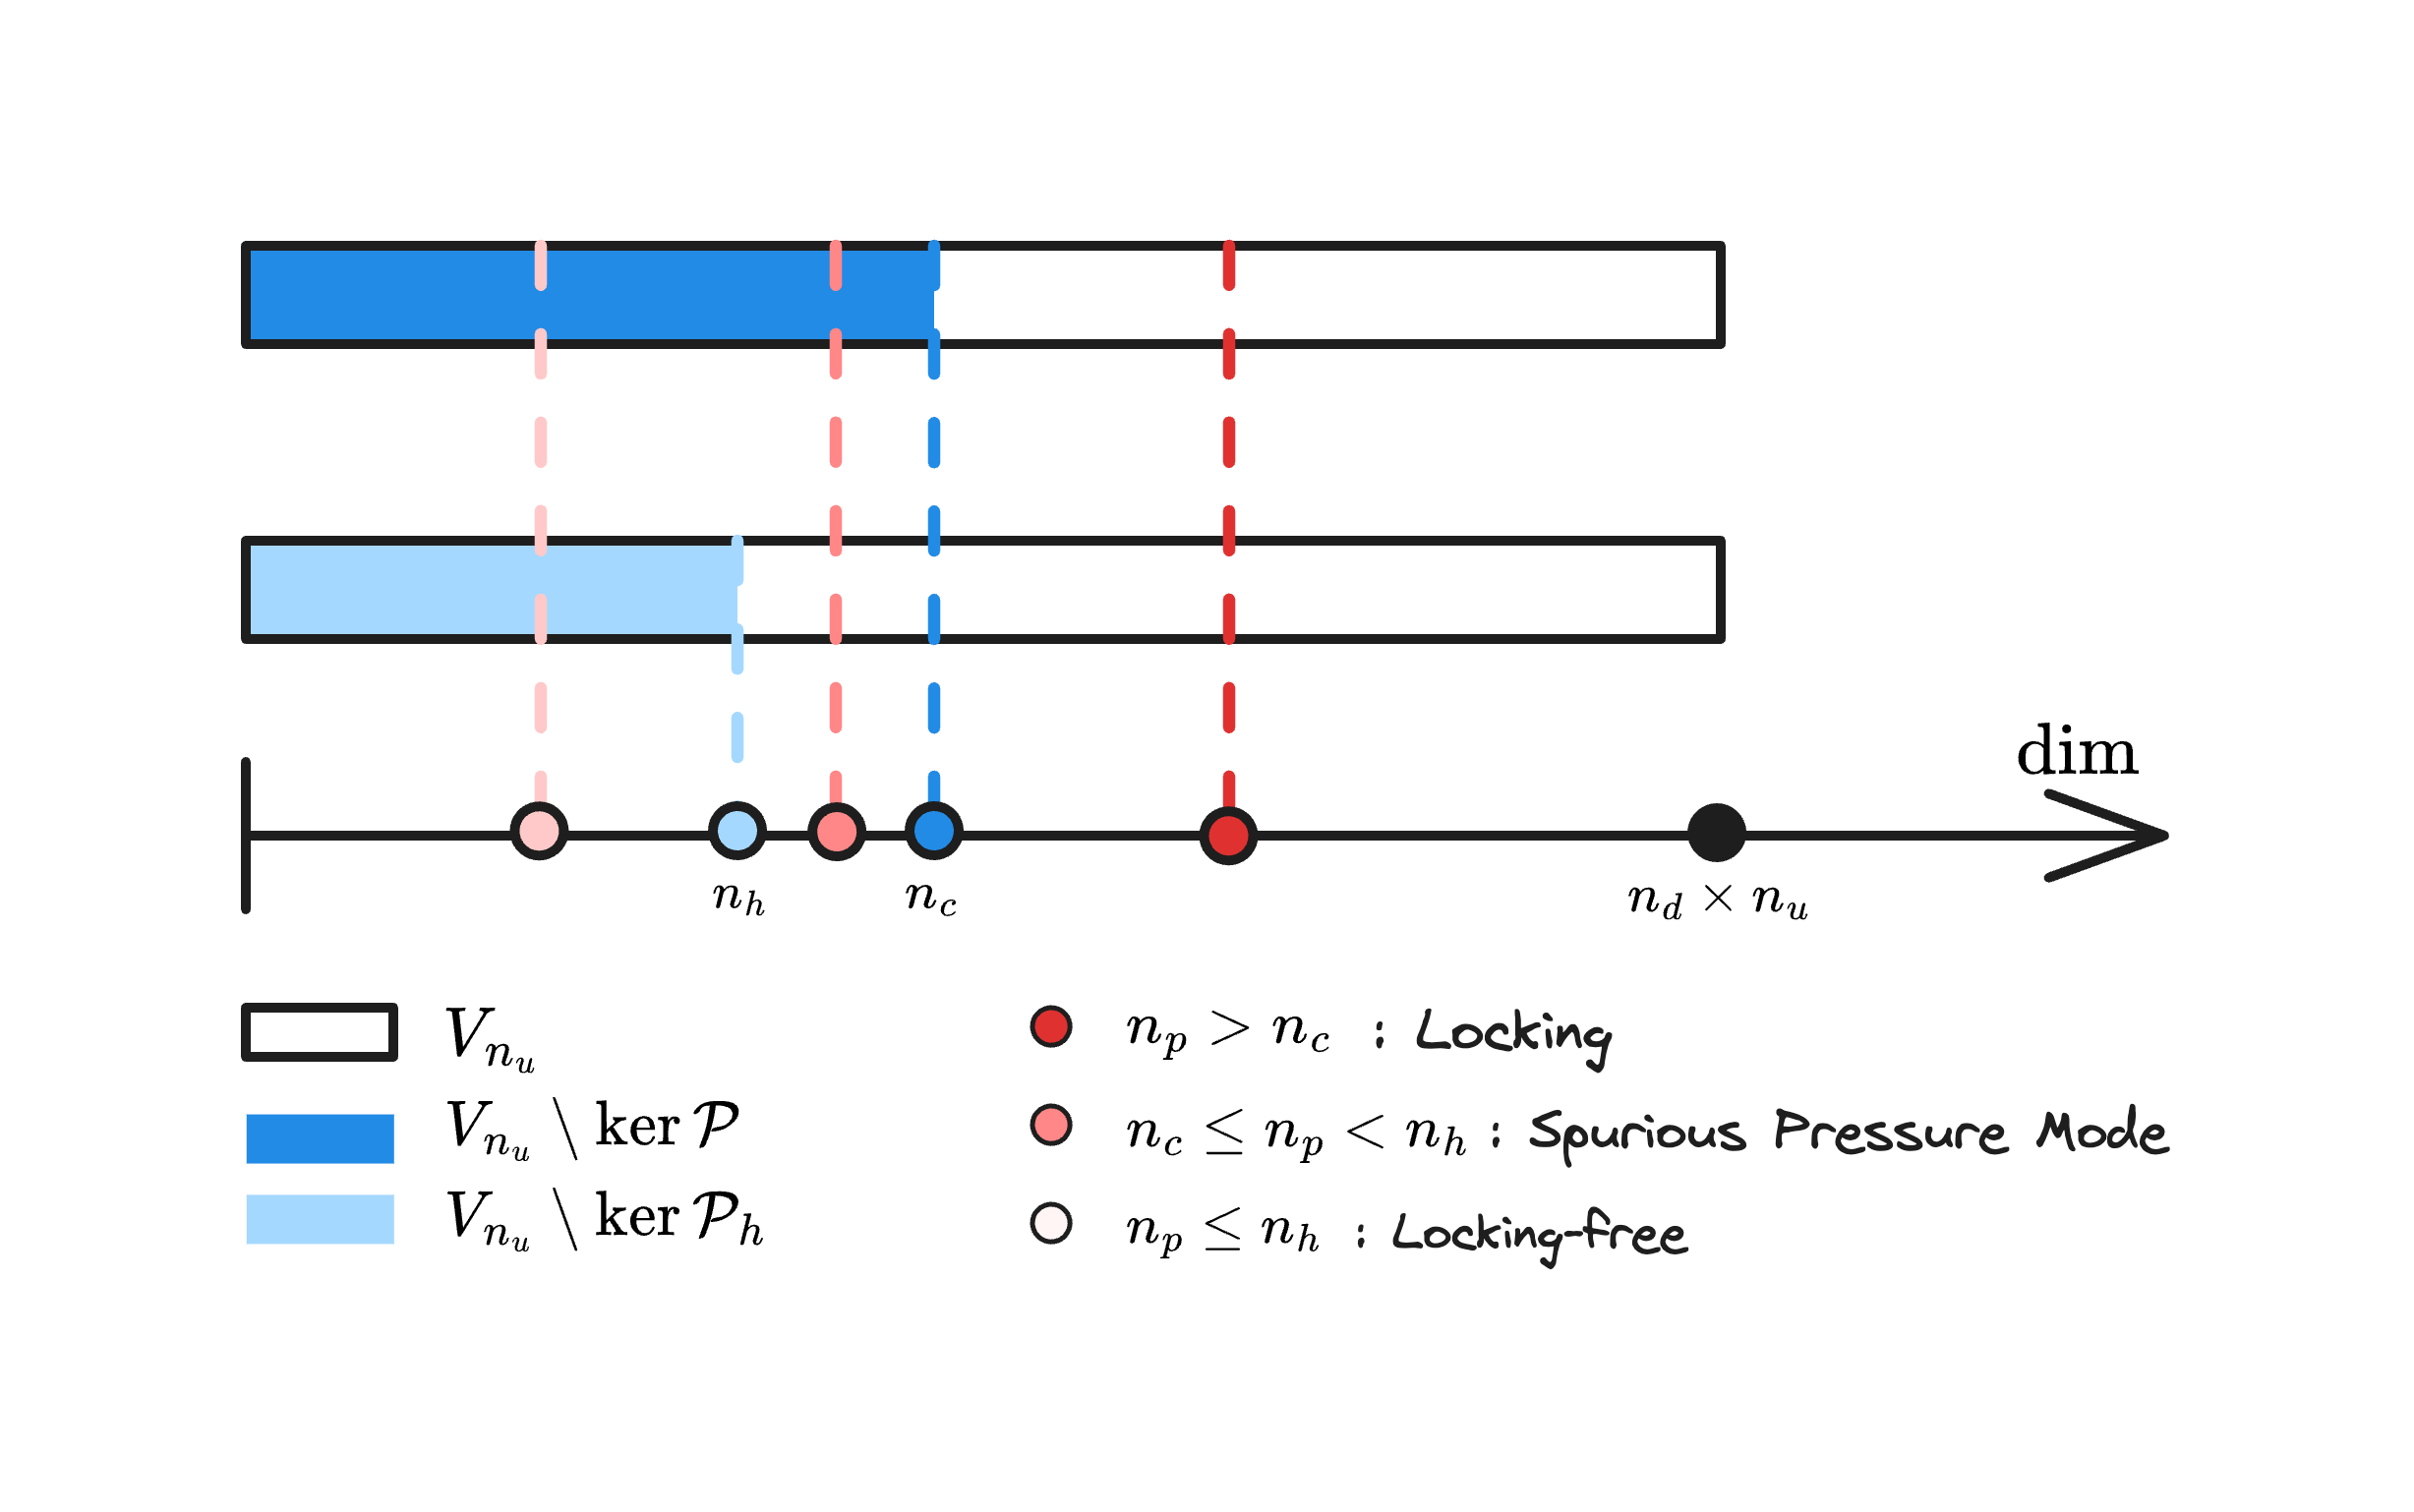
\includegraphics[width=0.8\textwidth]{png/space.png}
\caption{Illustration of estimator}\label{fg:space}
\end{figure}

Summarily, the formulation can satisfy the inf-sup condition and alleviate volumetric locking if at least the number of pressure nodes $n_p$ is less than $n_s$, so we name $n_s$ as the stabilized number of pressure nodes. At this moment, the volumetric constraint ratio should meet the following relation to ensure the inf-sup condition:
\begin{equation}\label{optimal_ratio}
r_{opt} \ge \frac{n_d \times n_u}{n_s}
\end{equation}

\begin{rmk}
Some uniform elements with special arrangements, like the union-jack element arrangement for 3-node triangular elements, can pass the inf-sup test \cite{chapelle1993}, but their pressure DOFs number is greater than $n_s$. This is because the union-jack arrangement leads to a lower nonzero eigenvalue number of $\tilde{a}$ and $a$ in Eq. \eqref{weak_penalty}, and the corresponding nonzero eigenvalue number is less than or equal to the stabilized number $n_s$, satisfying Eq. \eqref{optimal_ratio}. The similar cases about this special element arrangement are too few, so it is more straightforward to use the number of pressure nodes $n_p$ to measure $\dim (V_{n_u} \setminus \ker \mathcal{P}_h \mathcal{I}_h)$.
\end{rmk}

\begin{rmk}
It is obvious that the traditional optimal constraint ratio cannot fulfill this condition. However, not all formulations satisfying this condition can totally avoid volumetric locking. This is because $n_p \le n_s$ is not equivalent to $V_{n_u} \setminus \ker \mathcal{P}_h \mathcal{I}_h \subset V_{n_u} \setminus \ker \mathcal{P}$. Fortunately, well-posed nodal distributions of displacement and pressure can ensure this, which will be evidenced by numerical examples in the subsequent sections.
\end{rmk}

\subsection{Optimal volumetric constraint ratio}
The fulfillment of the inf-sup condition should require the number of pressure nodes $n_p$ to be lower than the stabilized number $n_s$, and now, we will demonstrate how to determine $n_s$ for a specific number of displacement DOFs.

In the 2D case, for instance, we first consider the linear polynomial displacement space $V_3$ that is given by:
\begin{equation}
V_3 = \mathrm{span} \left\{
\begin{pmatrix} 1 \\ 0 \end{pmatrix},
\begin{pmatrix} 0 \\ 1 \end{pmatrix},
\begin{pmatrix} x \\ 0 \end{pmatrix},
\begin{pmatrix} 0 \\ x \end{pmatrix},
\begin{pmatrix} y \\ 0 \end{pmatrix},
\begin{pmatrix} 0 \\ y \end{pmatrix}
\right\}
\end{equation}
or rearranged as follows,
\begin{equation}\label{base1}
V_3 = \mathrm{span}
\begin{Bmatrix}
\underbrace{
\begin{pmatrix} 1 \\ 0 \end{pmatrix},
\begin{pmatrix} 0 \\ 1 \end{pmatrix},
\begin{pmatrix} y \\ 0 \end{pmatrix},
\begin{pmatrix} 0 \\ x \end{pmatrix},
\begin{pmatrix} x \\ -y \end{pmatrix}
}_{\ker \mathcal{P}},
\underbrace{
\begin{pmatrix} x \\ y \end{pmatrix}
}_{V_3 \setminus \ker \mathcal{P}}
\end{Bmatrix}
\end{equation}
It can be counted that, for $n_u = 3$, $n_s = 1$. Following the path, the displacement space with a quadratic polynomial base, namely $V_6$, can be stated as:
\begin{equation}\label{base2}
V_6 = \mathrm{span}
\begin{Bmatrix}
\overbrace{
\begin{pmatrix} 1 \\ 0 \end{pmatrix},
\begin{pmatrix} 0 \\ 1 \end{pmatrix},
\begin{pmatrix} y \\ 0 \end{pmatrix},
\begin{pmatrix} 0 \\ x \end{pmatrix},
\begin{pmatrix} x \\ -y \end{pmatrix},
\begin{pmatrix} x^2 \\ -2xy \end{pmatrix},
\begin{pmatrix} y^2 \\ 0 \end{pmatrix},
\begin{pmatrix} 0 \\ x^2 \end{pmatrix},
\begin{pmatrix} -2xy \\ y^2 \end{pmatrix}
}^{\ker \mathcal{P}}, \\
\underbrace{
\begin{pmatrix} x \\ y \end{pmatrix},
\begin{pmatrix} x^2 \\ 2xy \end{pmatrix},
\begin{pmatrix} 2xy \\ y^2 \end{pmatrix}
}_{V_6 \setminus \ker \mathcal{P}}
\end{Bmatrix}
\end{equation}
In this circumstance, $n_s = 3$. As the order of the polynomial space increases, the optimal numbers of constraint DOFs for each order of the polynomial space are listed in Table. \ref{tab:constraint}, in which $n$ denotes the order of space $P_{n_u}$. For the flexibility of usage, the relation between $n_u$ and $n_s$ is summarized as follows:

\begin{equation}
n_s = \frac{n(n + 1)}{2}, \quad
n = \left\lfloor \frac{\sqrt{1 + 8n_u} - 3}{2} \right\rfloor
\end{equation}

\begin{table}[ht!]
\centering
\caption{Relationship between the number of displacement nodes $n_u$ and stabilized number of pressure nodes $n_s$}
\label{tab:constraint}
\begin{tabular}{ccccc}
\toprule
& \multicolumn{2}{c}{2D} & \multicolumn{2}{c}{3D} \\
$n$ & $n_u$ & $n_s$ & $n_u$ & $n_s$ \\
\midrule
1 & 3 & 1 & 4 & 1 \\
2 & 6 & 3 & 10 & 4 \\
3 & 10 & 6 & 20 & 10 \\
4 & 15 & 10 & 35 & 20 \\
\vdots & \vdots & \vdots & \vdots & \vdots \\
\bottomrule
\end{tabular}
\end{table}

For the 3D case, following the path in 2D, the linear polynomial space $V_4$ is considered herein, and the arranged space of $V_4$ is listed as follows:
\begin{equation}
V_4 = \mathrm{span}
\begin{Bmatrix}
\overbrace{
\begin{pmatrix} 1 \\ 0 \\ 0 \end{pmatrix},
\begin{pmatrix} 0 \\ 1 \\ 0 \end{pmatrix},
\begin{pmatrix} 0 \\ 0 \\ 1 \end{pmatrix},
\begin{pmatrix} 0 \\ x \\ 0 \end{pmatrix},
\begin{pmatrix} 0 \\ 0 \\ x \end{pmatrix},
\begin{pmatrix} y \\ 0 \\ 0 \end{pmatrix}
}^{\ker \mathcal{P}},
\\
\underbrace{
\begin{pmatrix} 0 \\ 0 \\ y \end{pmatrix},
\begin{pmatrix} z \\ 0 \\ 0 \end{pmatrix},
\begin{pmatrix} 0 \\ z \\ 0 \end{pmatrix},
\begin{pmatrix} x \\ -y \\ 0 \end{pmatrix},
\begin{pmatrix} x \\ 0 \\ -z \end{pmatrix}
}_{\ker \mathcal{P}},
\underbrace{
\begin{pmatrix} x \\ y \\ z \end{pmatrix}
}_{V_{n_u} \setminus \ker \mathcal{P}}
\end{Bmatrix}
\end{equation}

For brevity, the stabilized numbers for higher-order polynomial displacement spaces are directly listed in Table. \ref{tab:constraint}, and it can be summarized that, for a given number of displacement DOFs, the stabilized number for pressure DOFs can be calculated as follows:
\begin{align}
n_s &= \frac{n(n + 1)(n + 2)}{6} \\
n &= \left\lfloor
\left( 3n_u + \frac{1}{3}\sqrt{81n_u^2 - \frac{1}{3}} \right)^{\frac{1}{3}}
+
\frac{1}{3\left( 3n_u + \frac{1}{3}\sqrt{81n_u^2 - \frac{1}{3}} \right)^{\frac{1}{3}}} - 2
\right\rfloor
\end{align}

% Table \ref{tb:inf_sup_condition} lists the effectiveness of the traditional constraint ratio and the proposed optimal constraint ratio for traditional mixed formulation schemes, comparing the constraint ratios with the fulfillment of the inf-sup condition using analytical proof and numerical prediction. The table reveals that the traditional constraint ratio $r \ge n_d$ is not sufficient to guarantee the inf-sup condition, especially for low-order mixed formulations like T3P1 and Q4P1. The proposed optimal constraint ratio $r_{opt} \ge \frac{n_d \times n_u}{n_s}$ is more effective in ensuring the inf-sup condition,
% since the corresponding results is consistent with numerical prediction or analytical proof of inf--sup condition.

% \begin{table}[!htb]
% \centering
% \caption{Constraint ratio and inf-sup condition for various mixed formulations} \label{tb:inf_sup_condition}
% \begin{tabular}{ccccc}
% \hline
% \multirow{2}{*}{\scriptsize Formulation} & {\scriptsize Constraint Ratio} & \multicolumn{2}{c}{\scriptsize Inf-sup condition} & {\scriptsize Constraint Ratio} \\
% & {\scriptsize $r \ge n_d$} & {\tiny Numerical prediction} & {\tiny Analytical proof} & {\scriptsize $r = r_{opt}$} \\
% \hline
% \parbox{0.2\textwidth}{\centering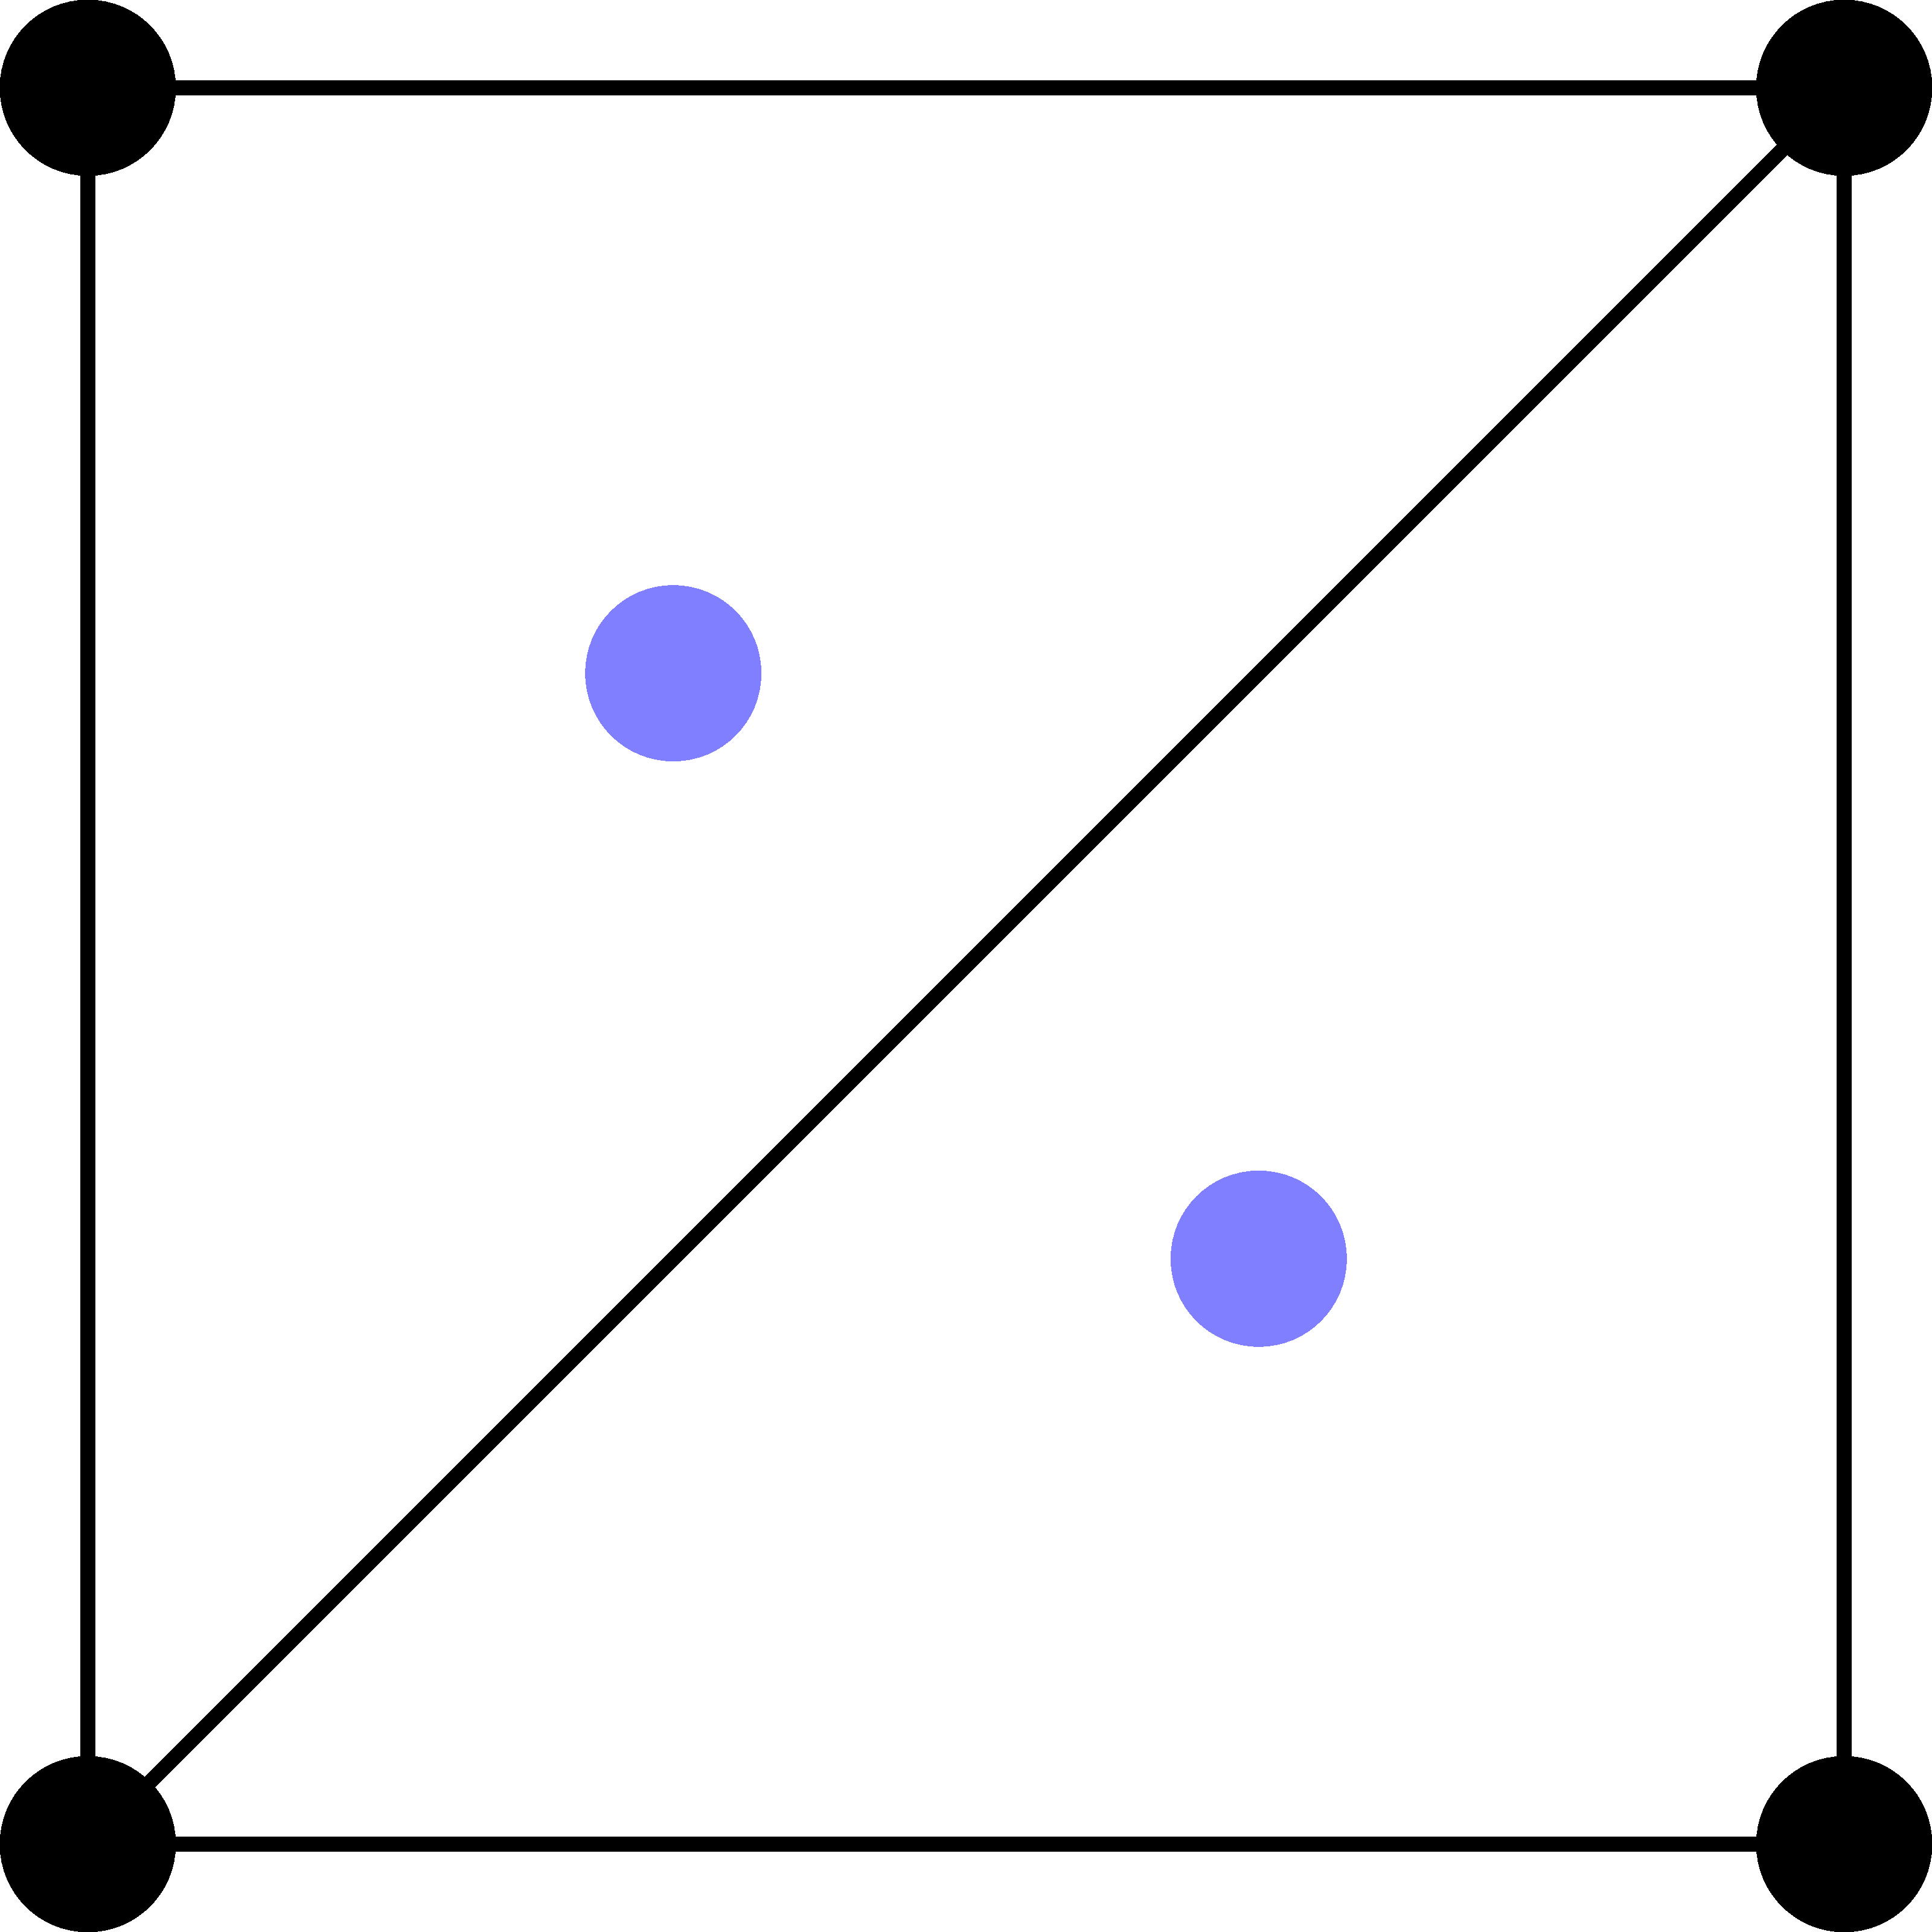
\includegraphics[width=0.1\textwidth]{png/mix_T3P1.png}\\[-1.5ex]{\tiny T3P1($r=1$)}\\[1ex]}
% & $\times$ & $\times$ & $\times$ & $\times$ \\
% \parbox{0.2\textwidth}{\centering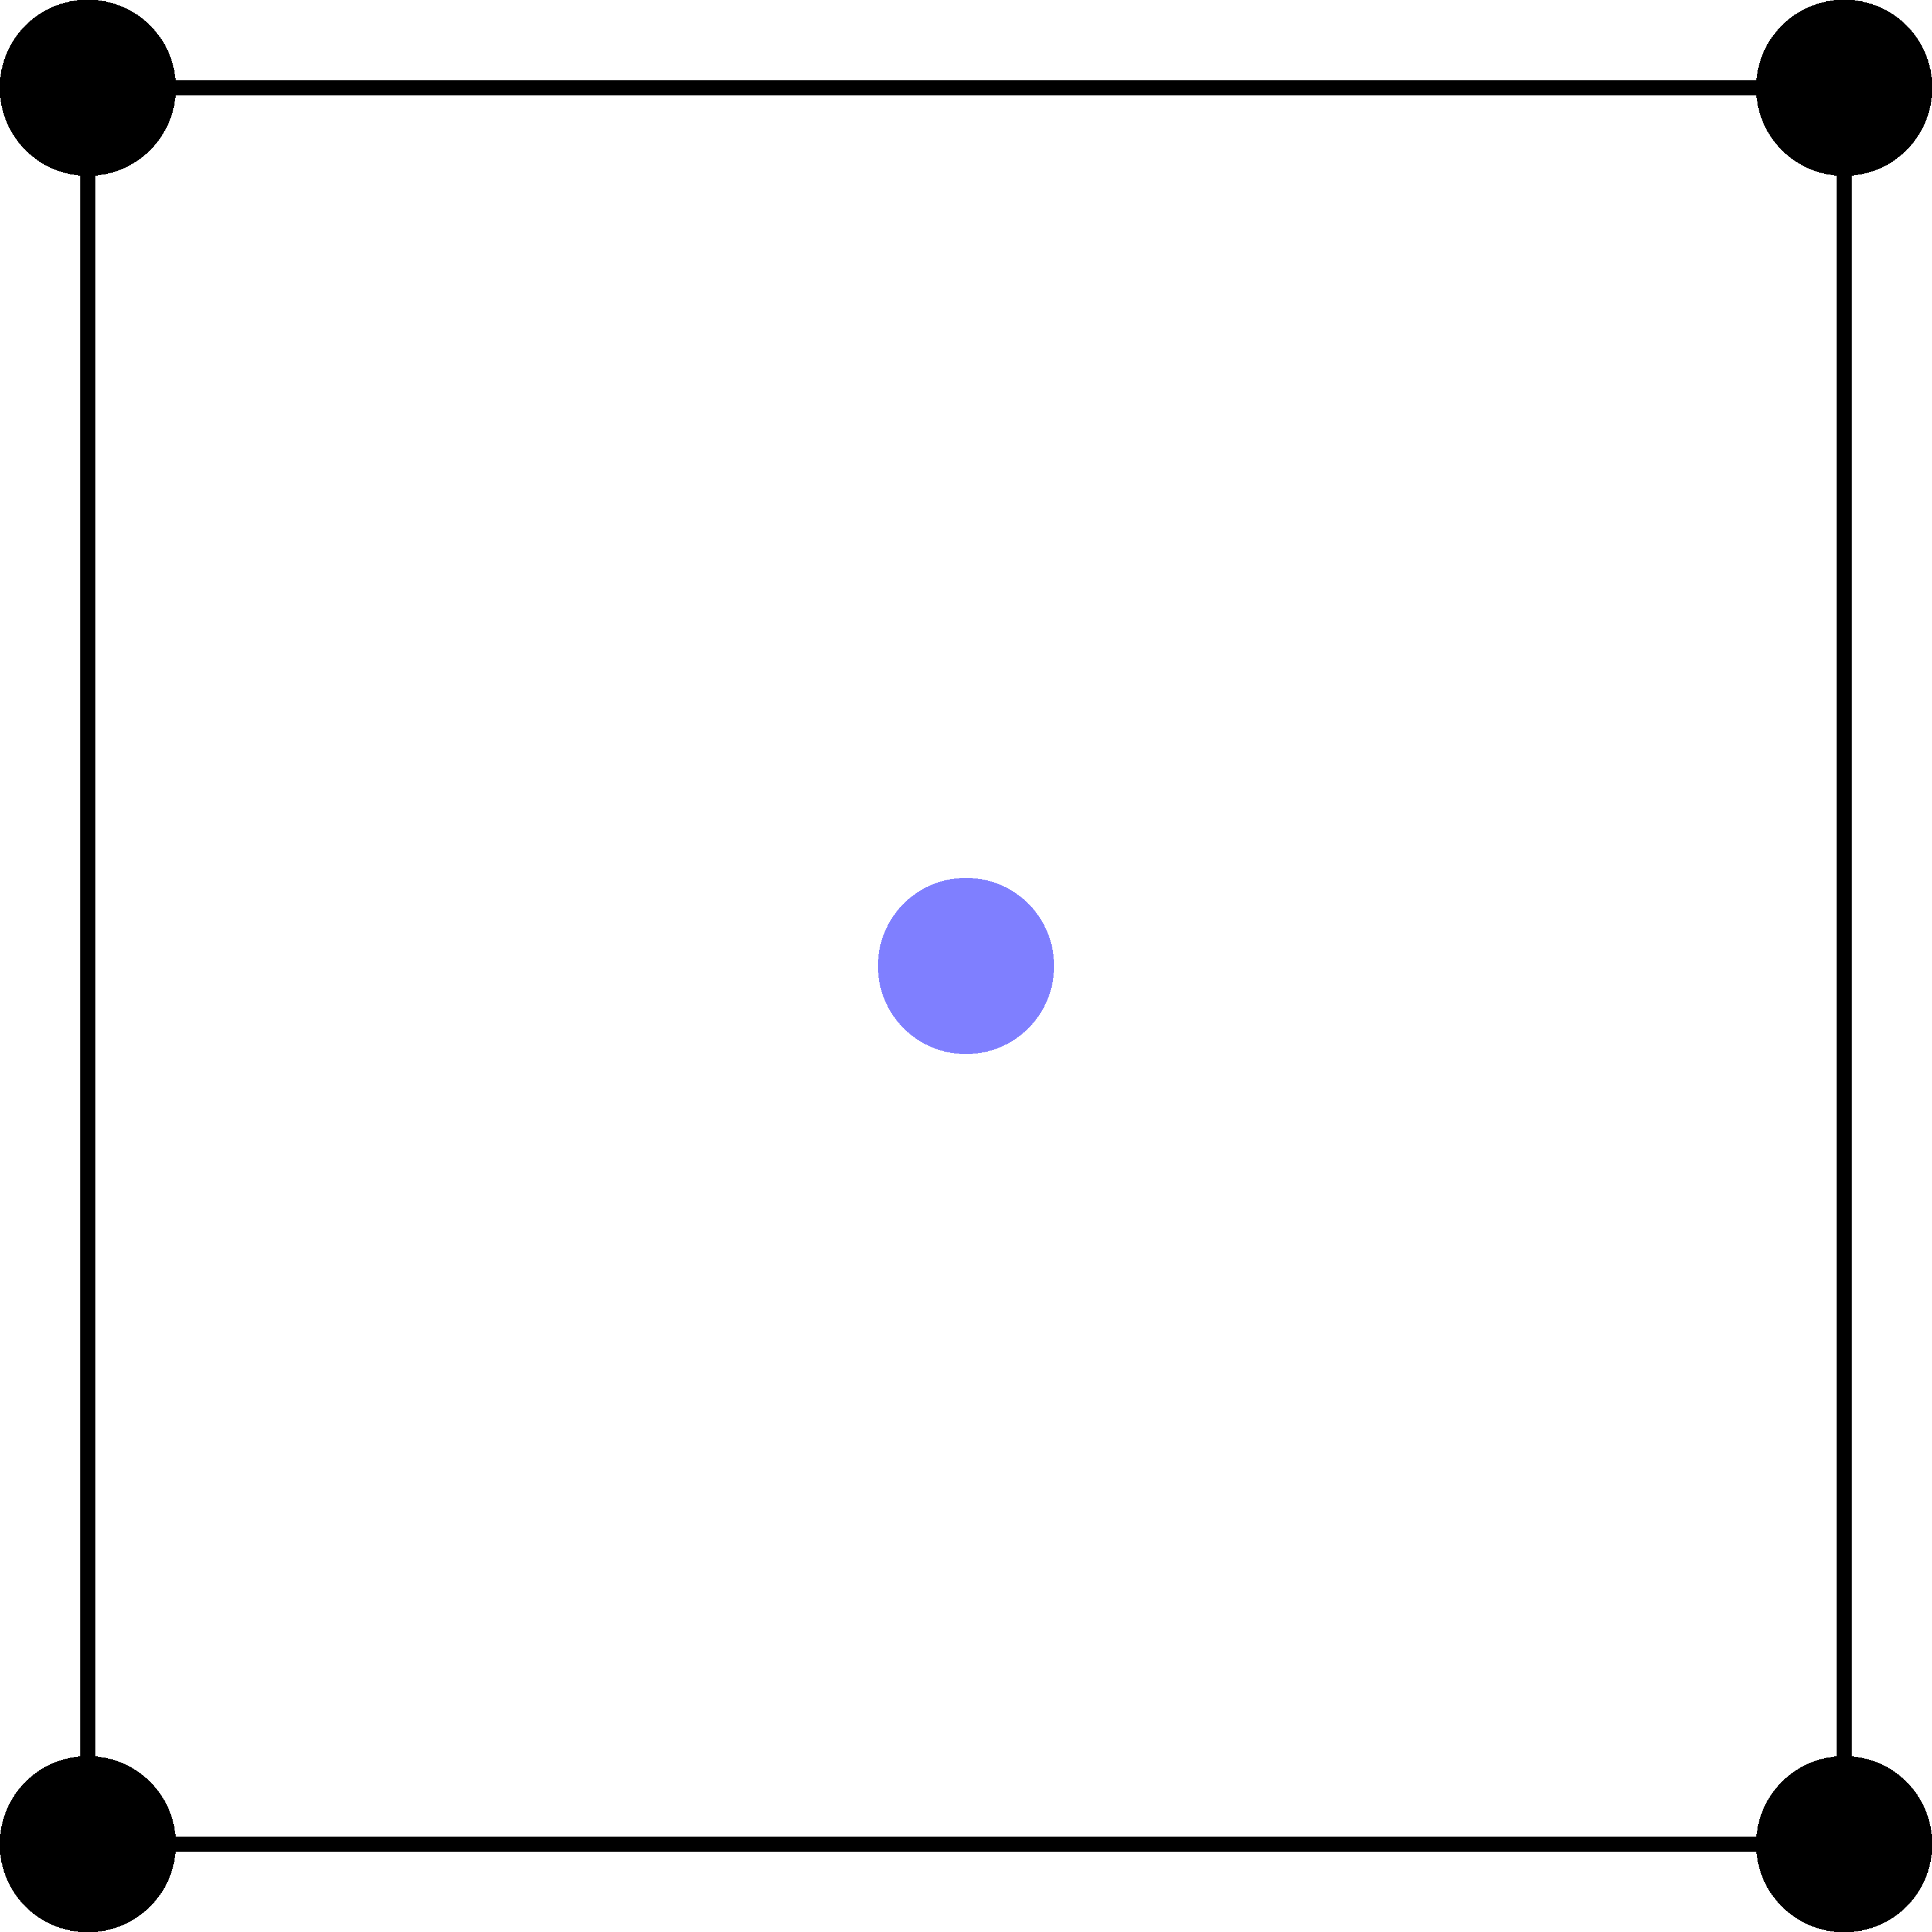
\includegraphics[width=0.1\textwidth]{png/mix_Q4P1.png}\\[-1.5ex]{\tiny Q4P1($r=2$)}\\[1ex]}
% & \checkmark & $\times$ & $\times$ & $\times$ \\
% \parbox{0.2\textwidth}{\centering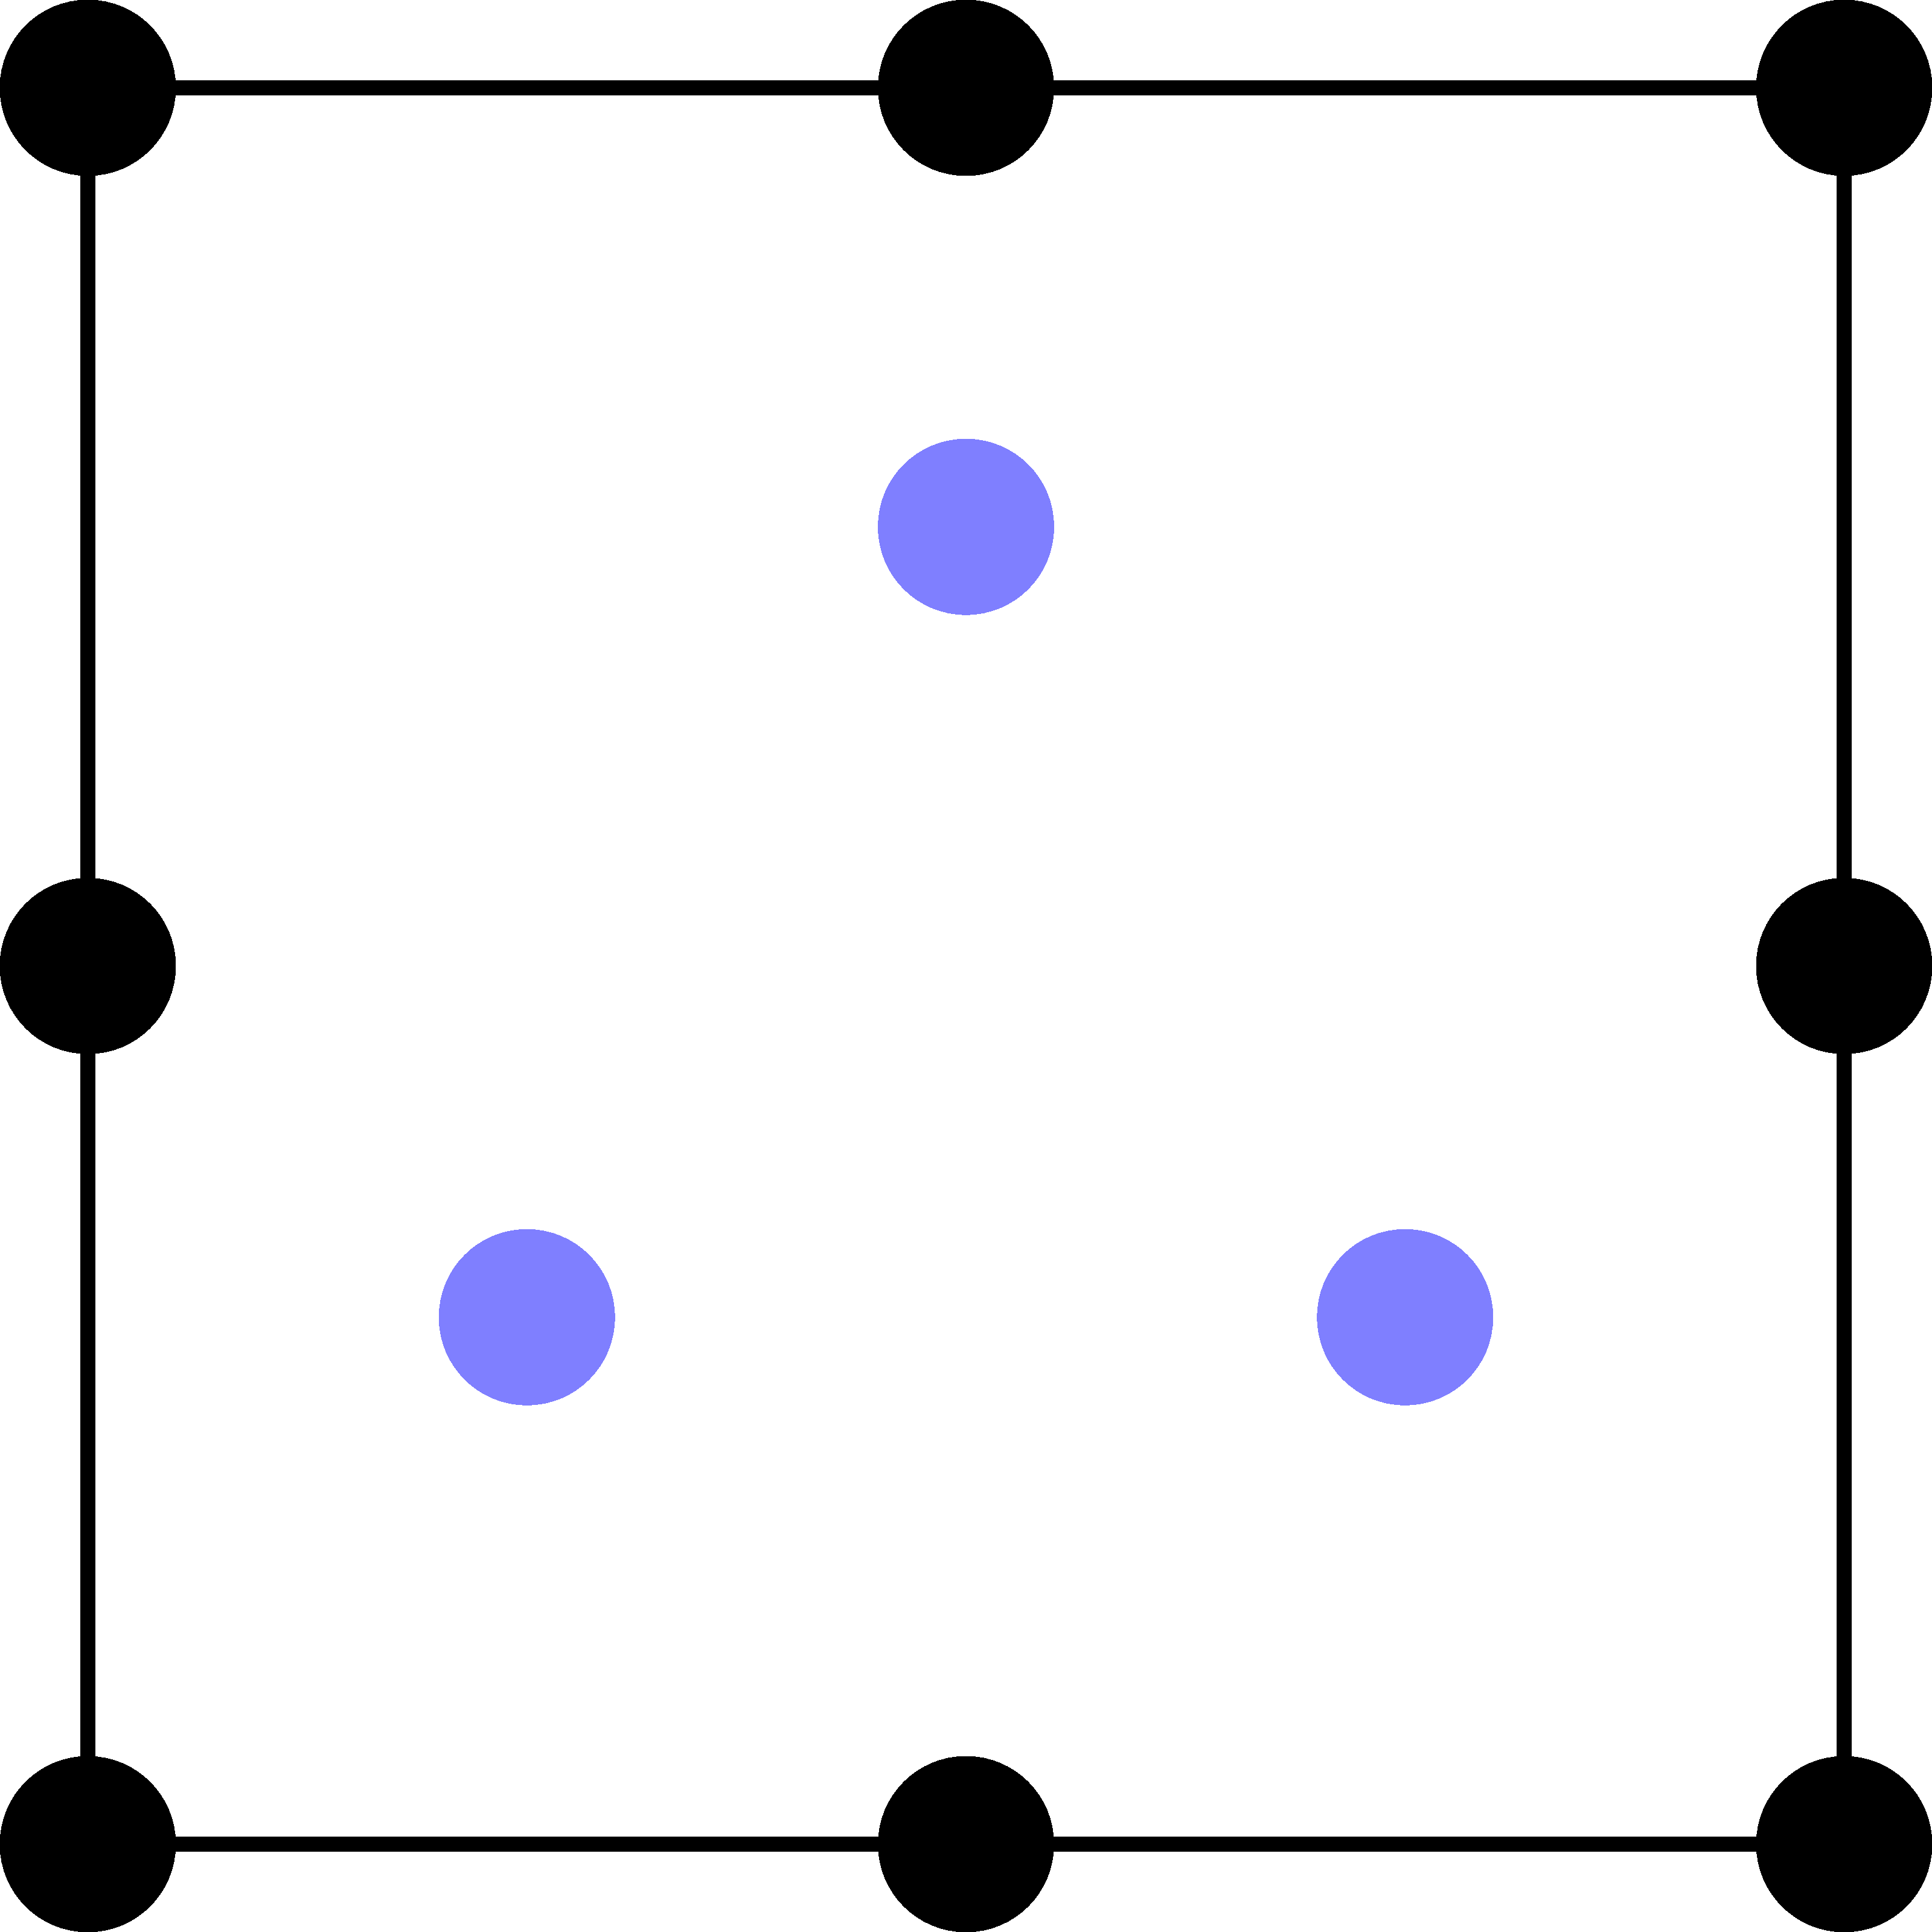
\includegraphics[width=0.1\textwidth]{png/mix_Q8P3.png}\\[-1.5ex]{\tiny Q8P3($r=2$)}\\[1ex]}
% & \checkmark & $\times$ & $\times$ & $\times$ \\
% \parbox{0.2\textwidth}{\centering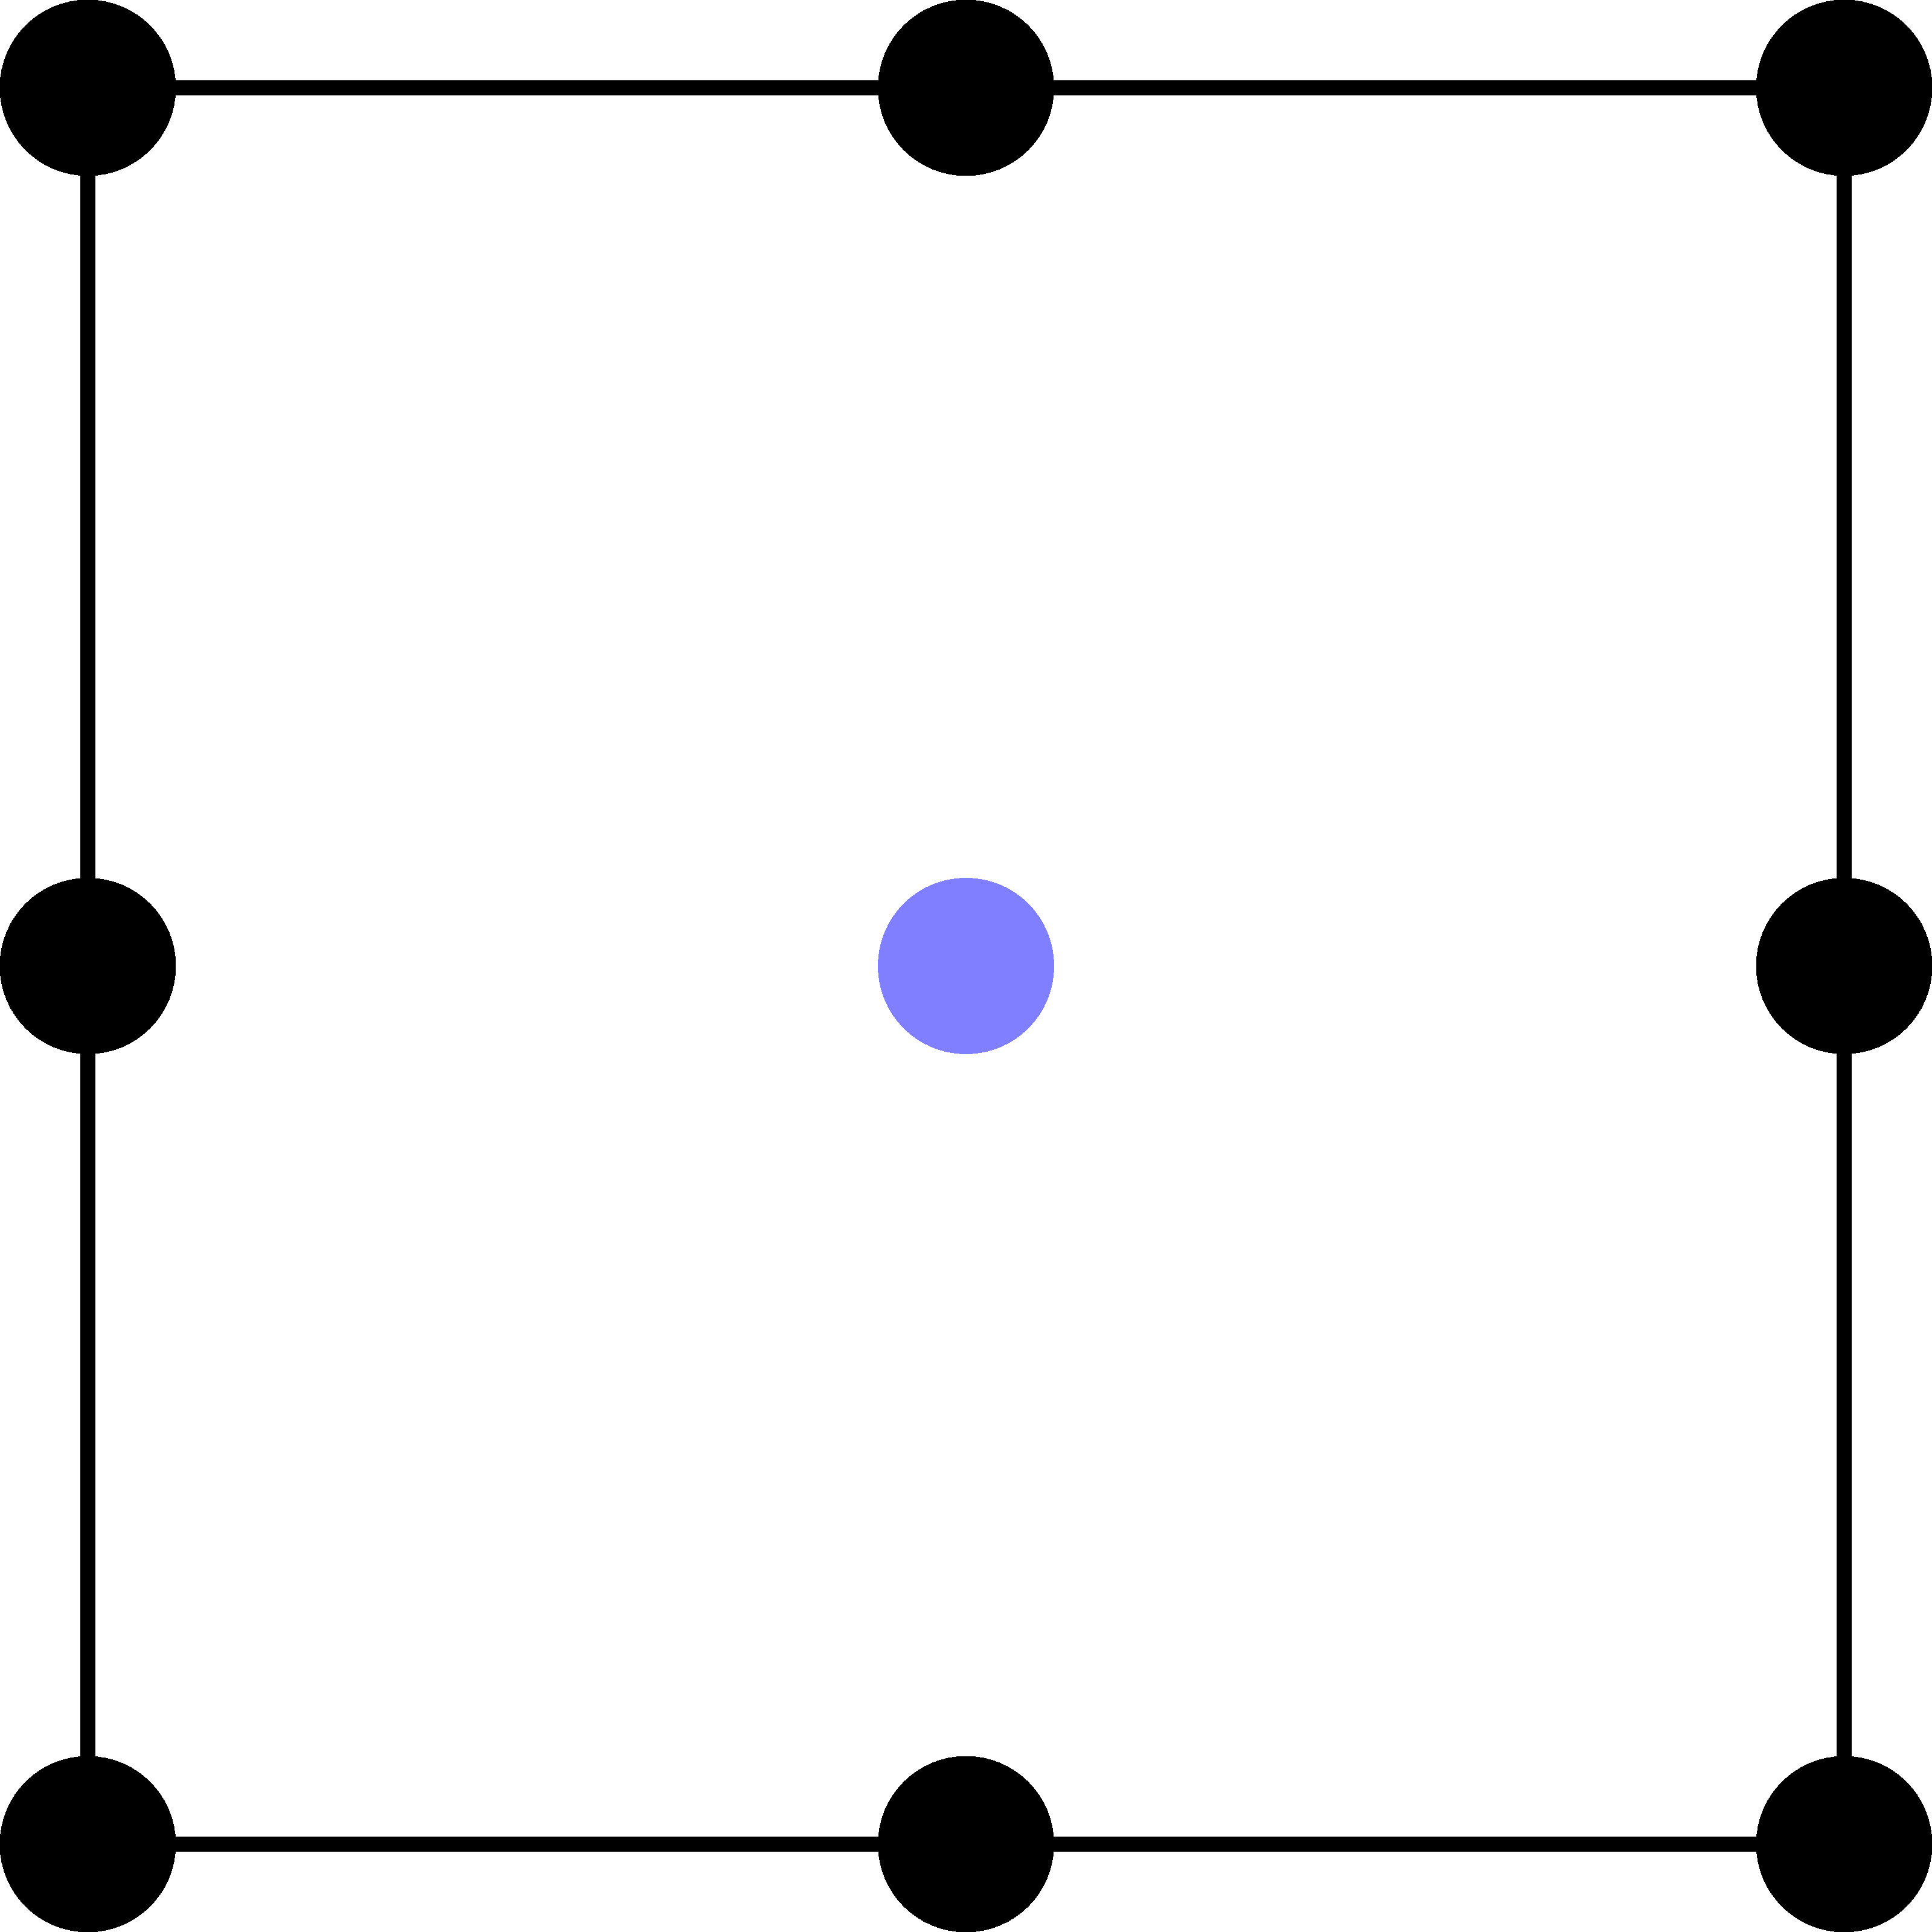
\includegraphics[width=0.1\textwidth]{png/mix_Q8P1.png}\\[-1.5ex]{\tiny Q8P1($r=6$)}\\[1ex]}
% & \checkmark & \checkmark & \checkmark & \checkmark \\
% \parbox{0.2\textwidth}{\centering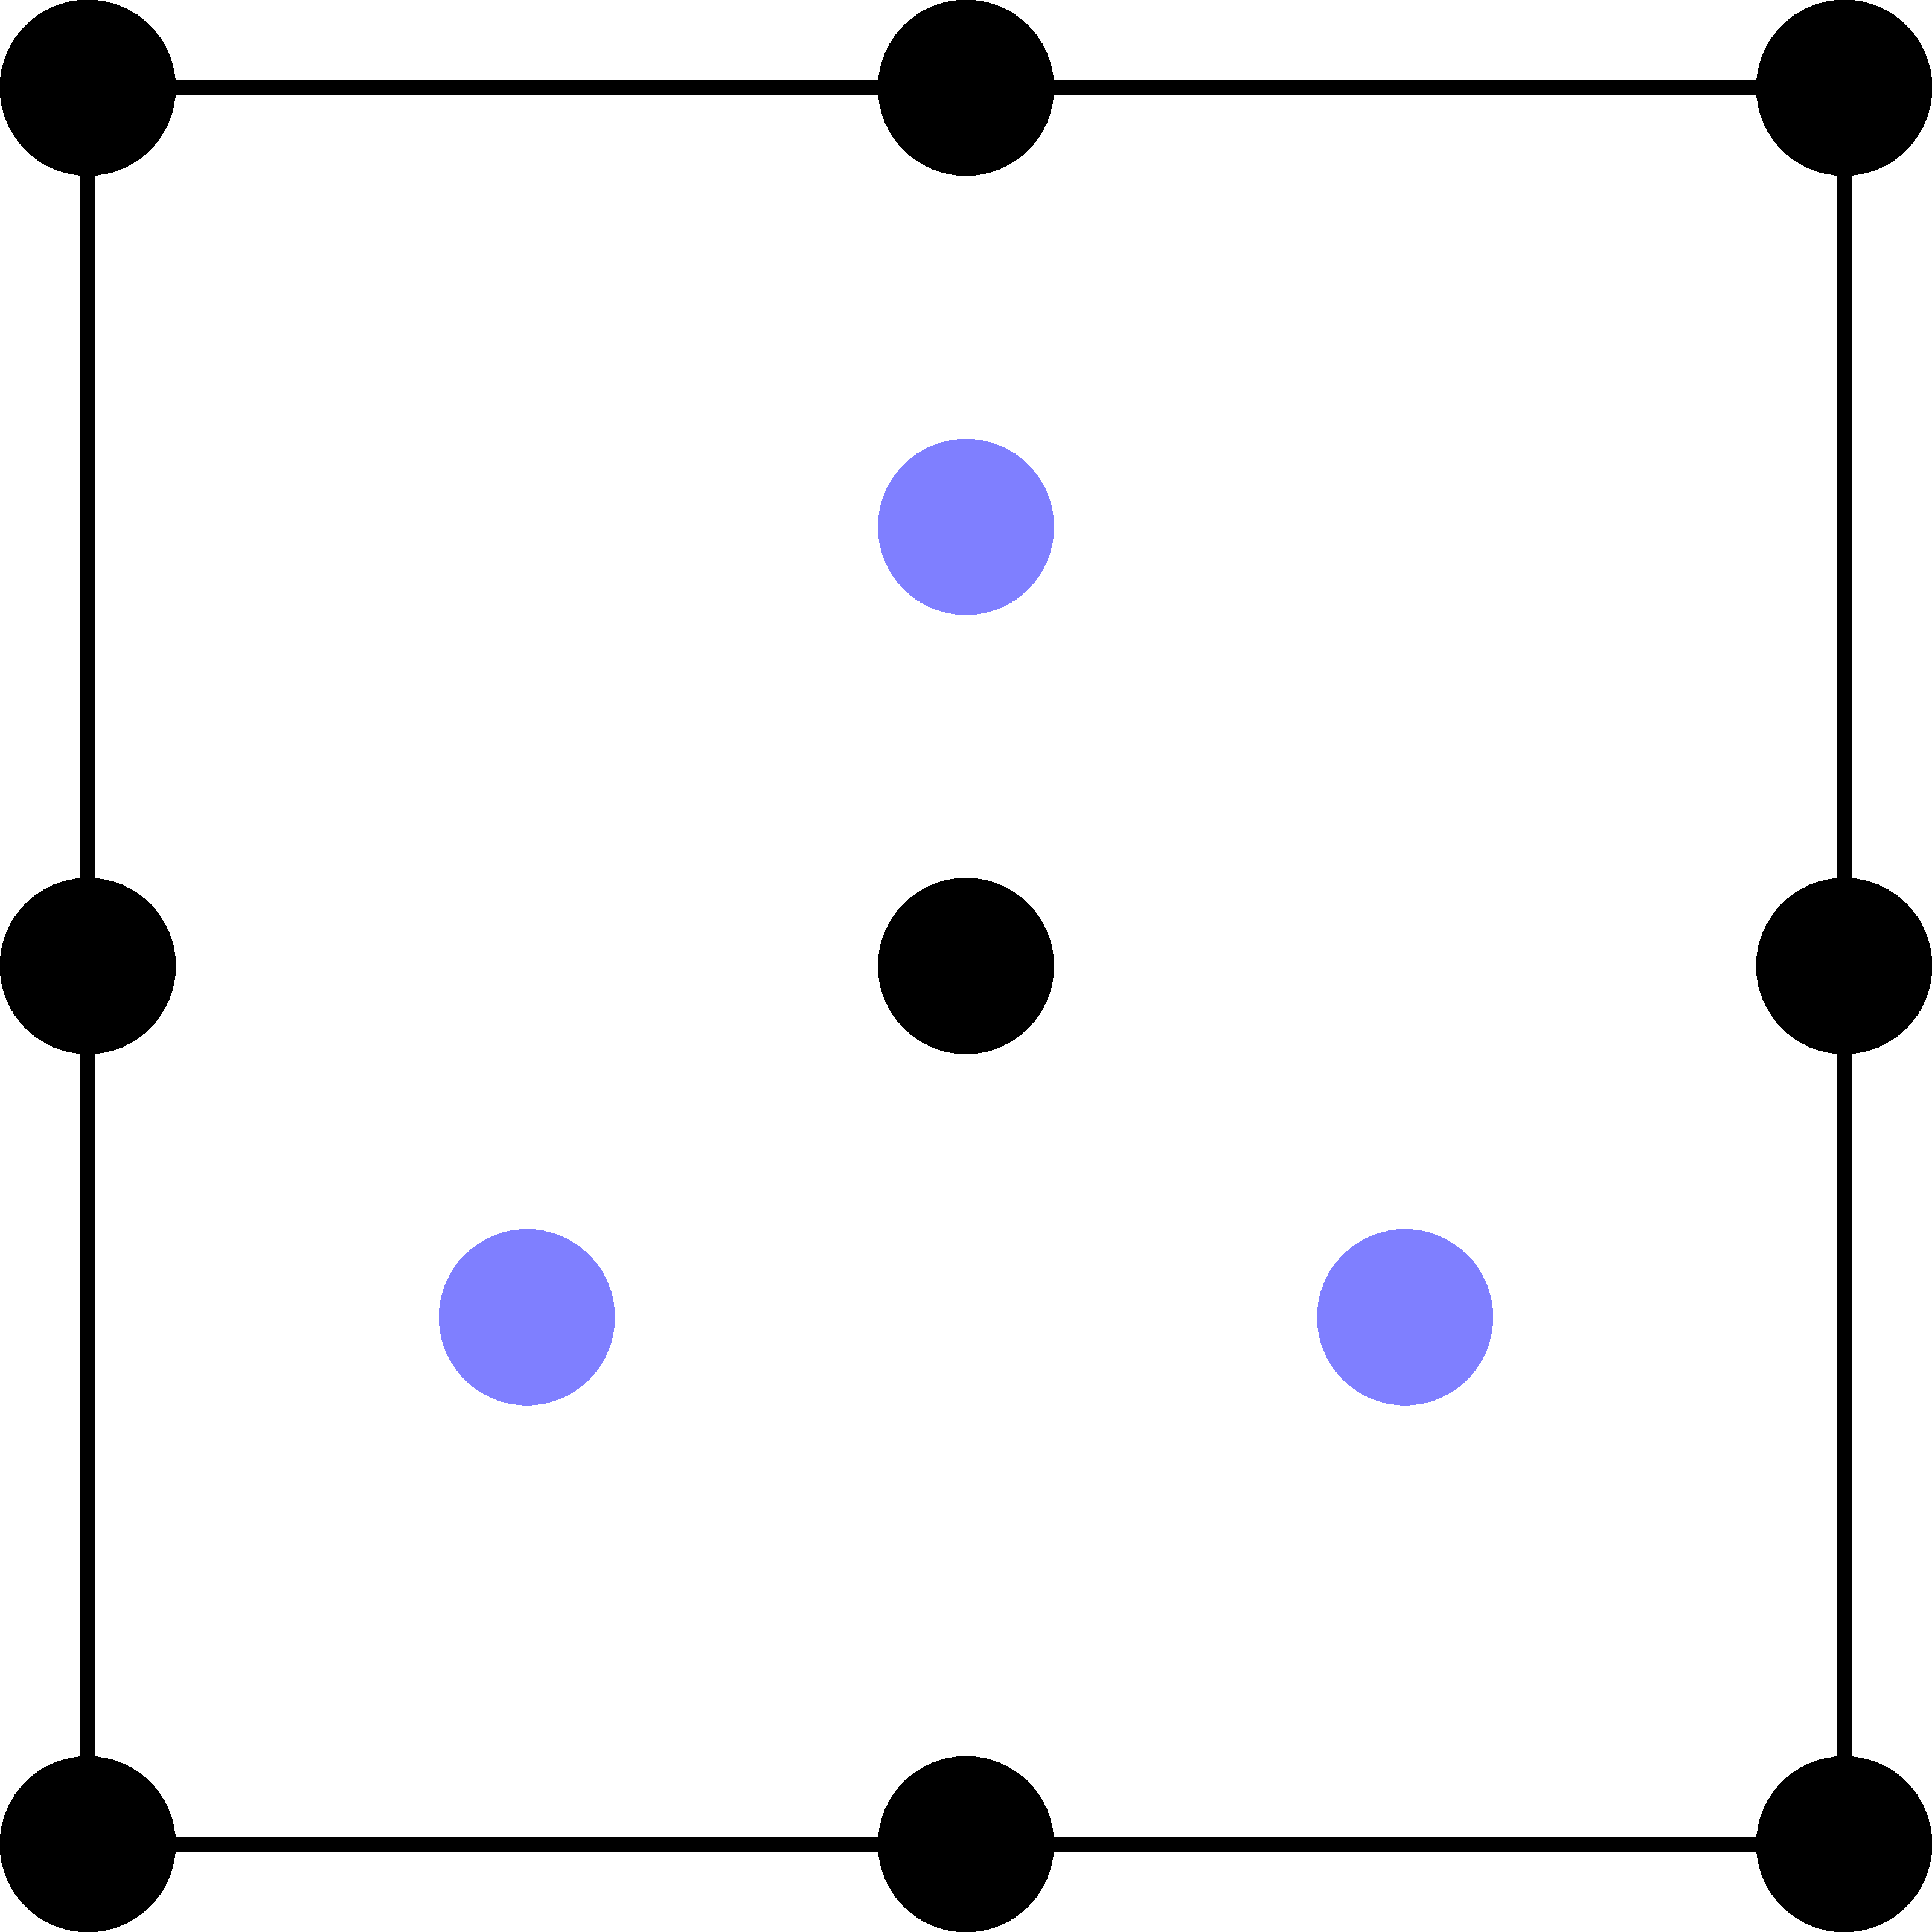
\includegraphics[width=0.1\textwidth]{png/mix_Q9P3.png}\\[-1.5ex]{\tiny Q9P3($r=\frac{8}{3}$)}\\[1ex]}
% & \checkmark & \checkmark & \checkmark & \checkmark \\
% \parbox{0.2\textwidth}{\centering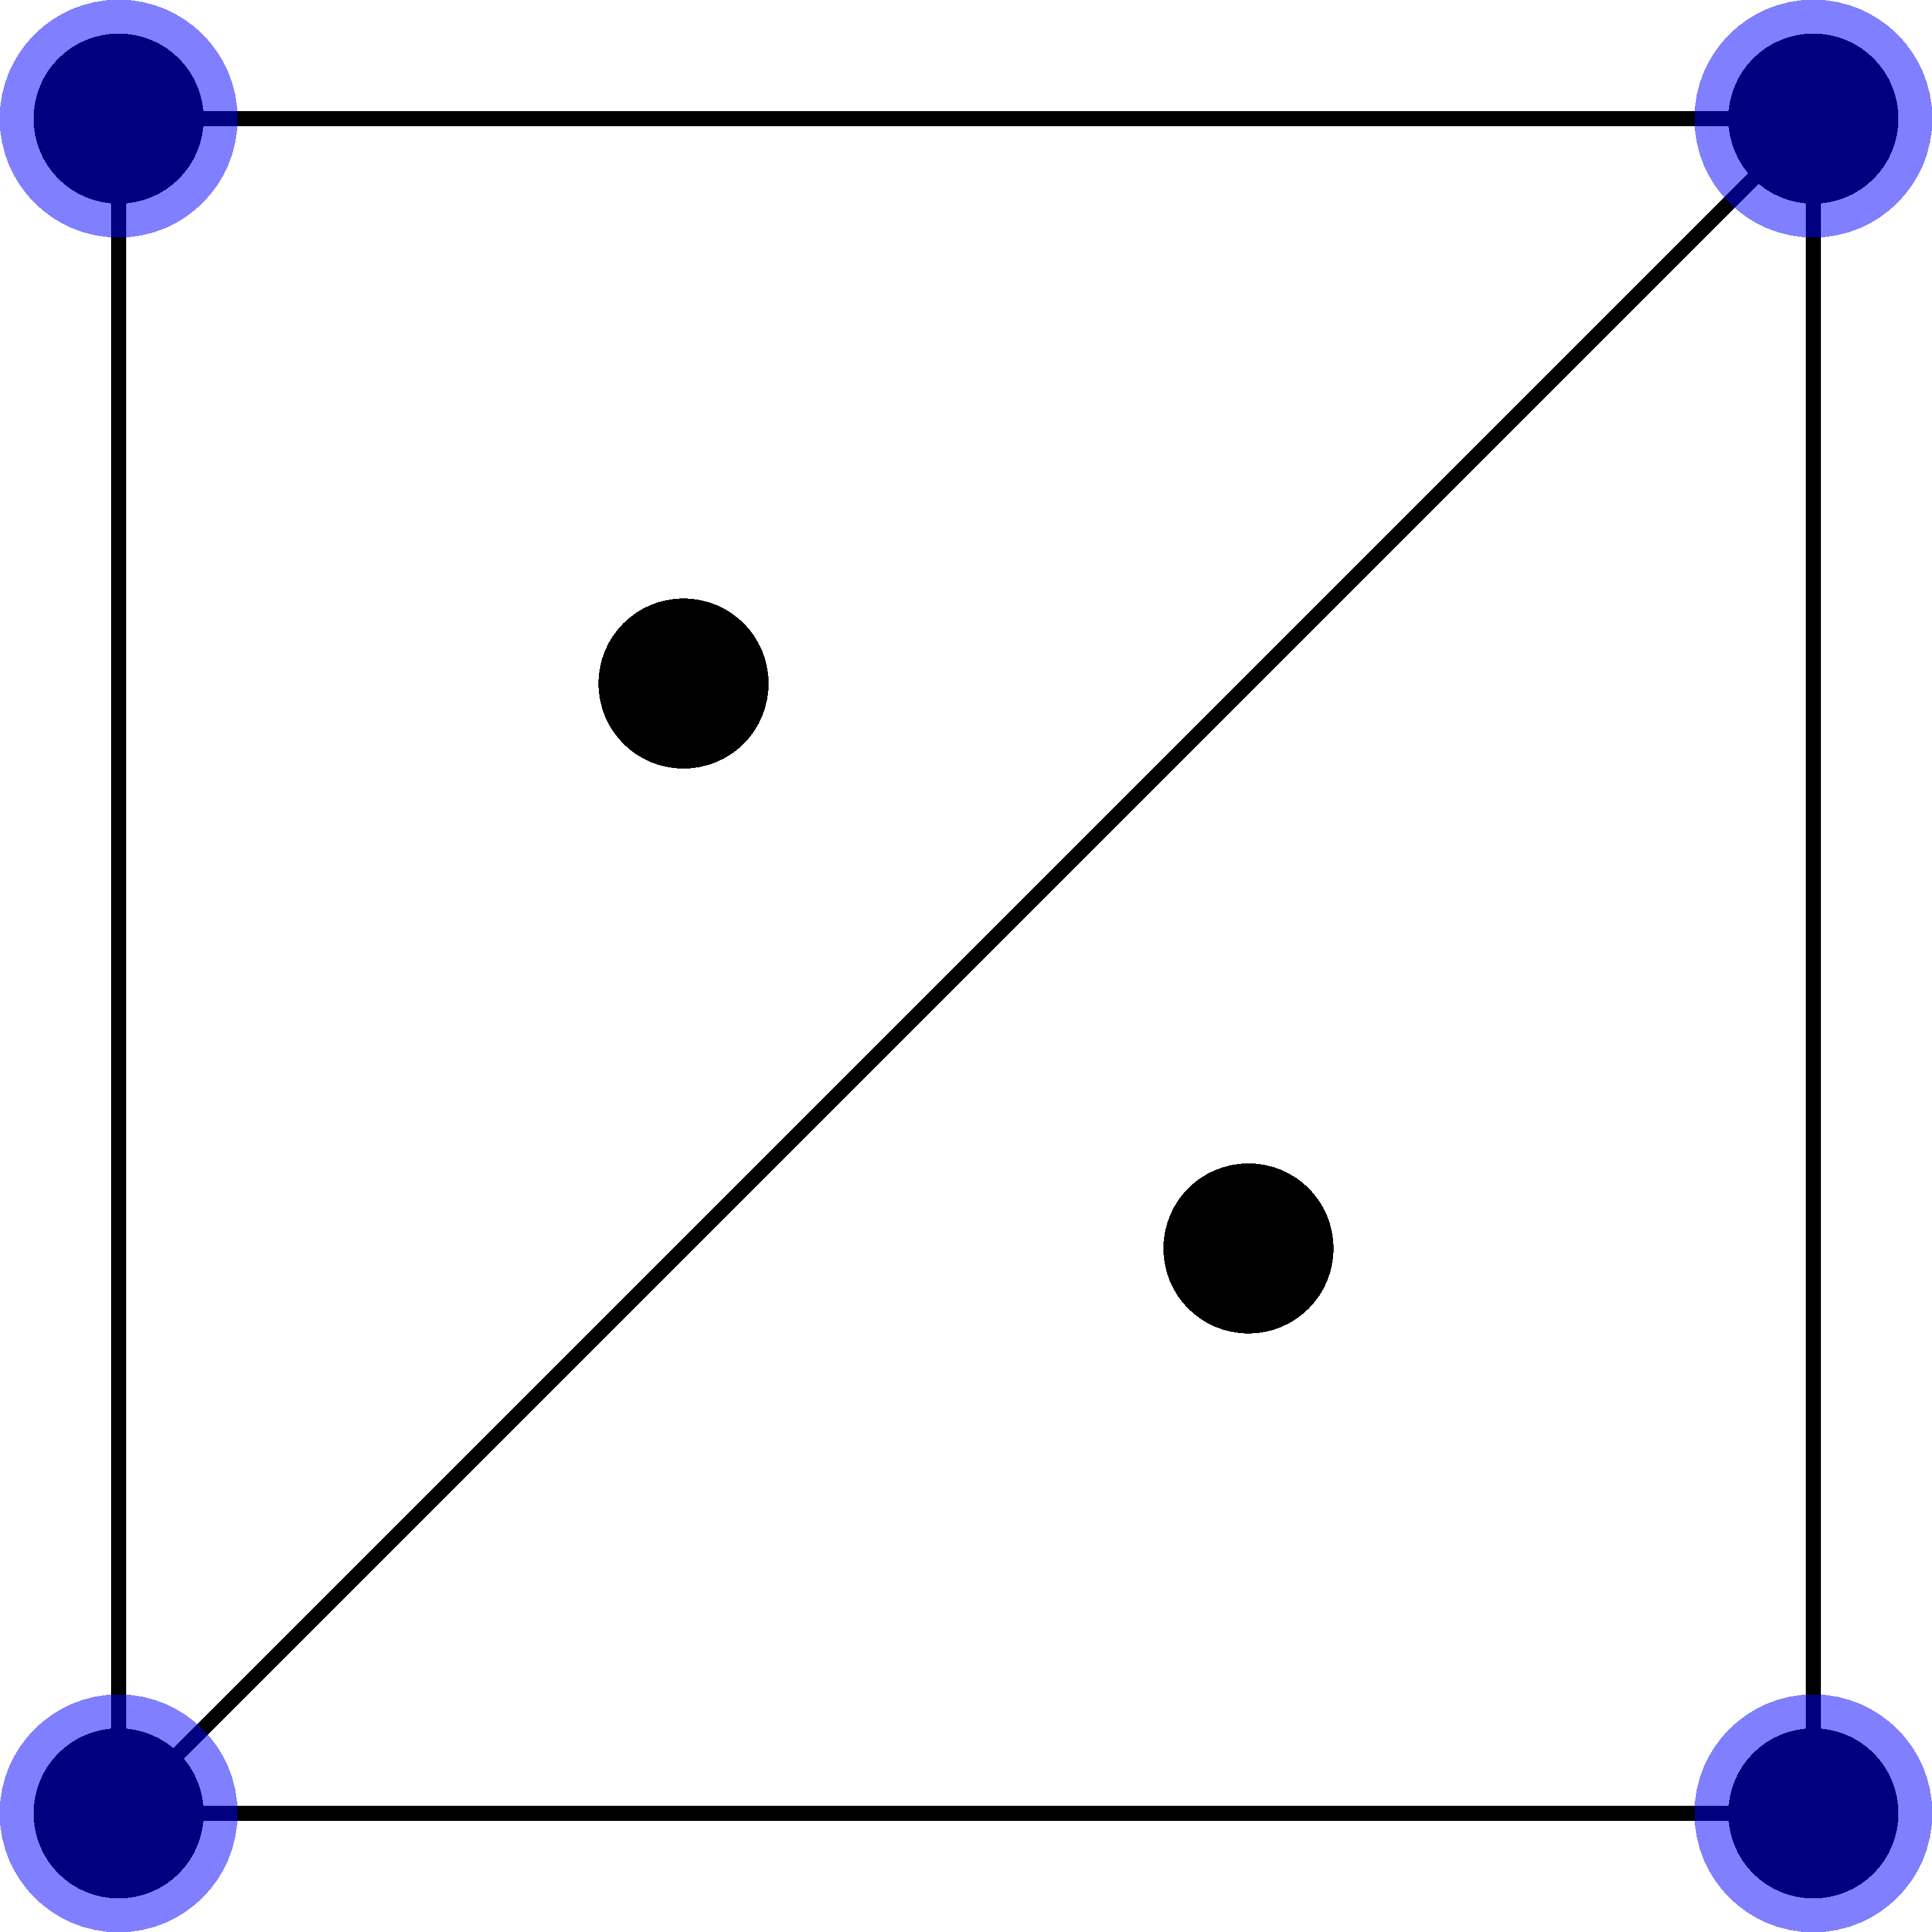
\includegraphics[width=0.1\textwidth]{png/mini.png}\\[-1.5ex]{\tiny MINI($r=\frac{8}{3}$)}\\[1ex]}
% & \checkmark & \checkmark & \checkmark & \checkmark \\
% \parbox{0.2\textwidth}{\centering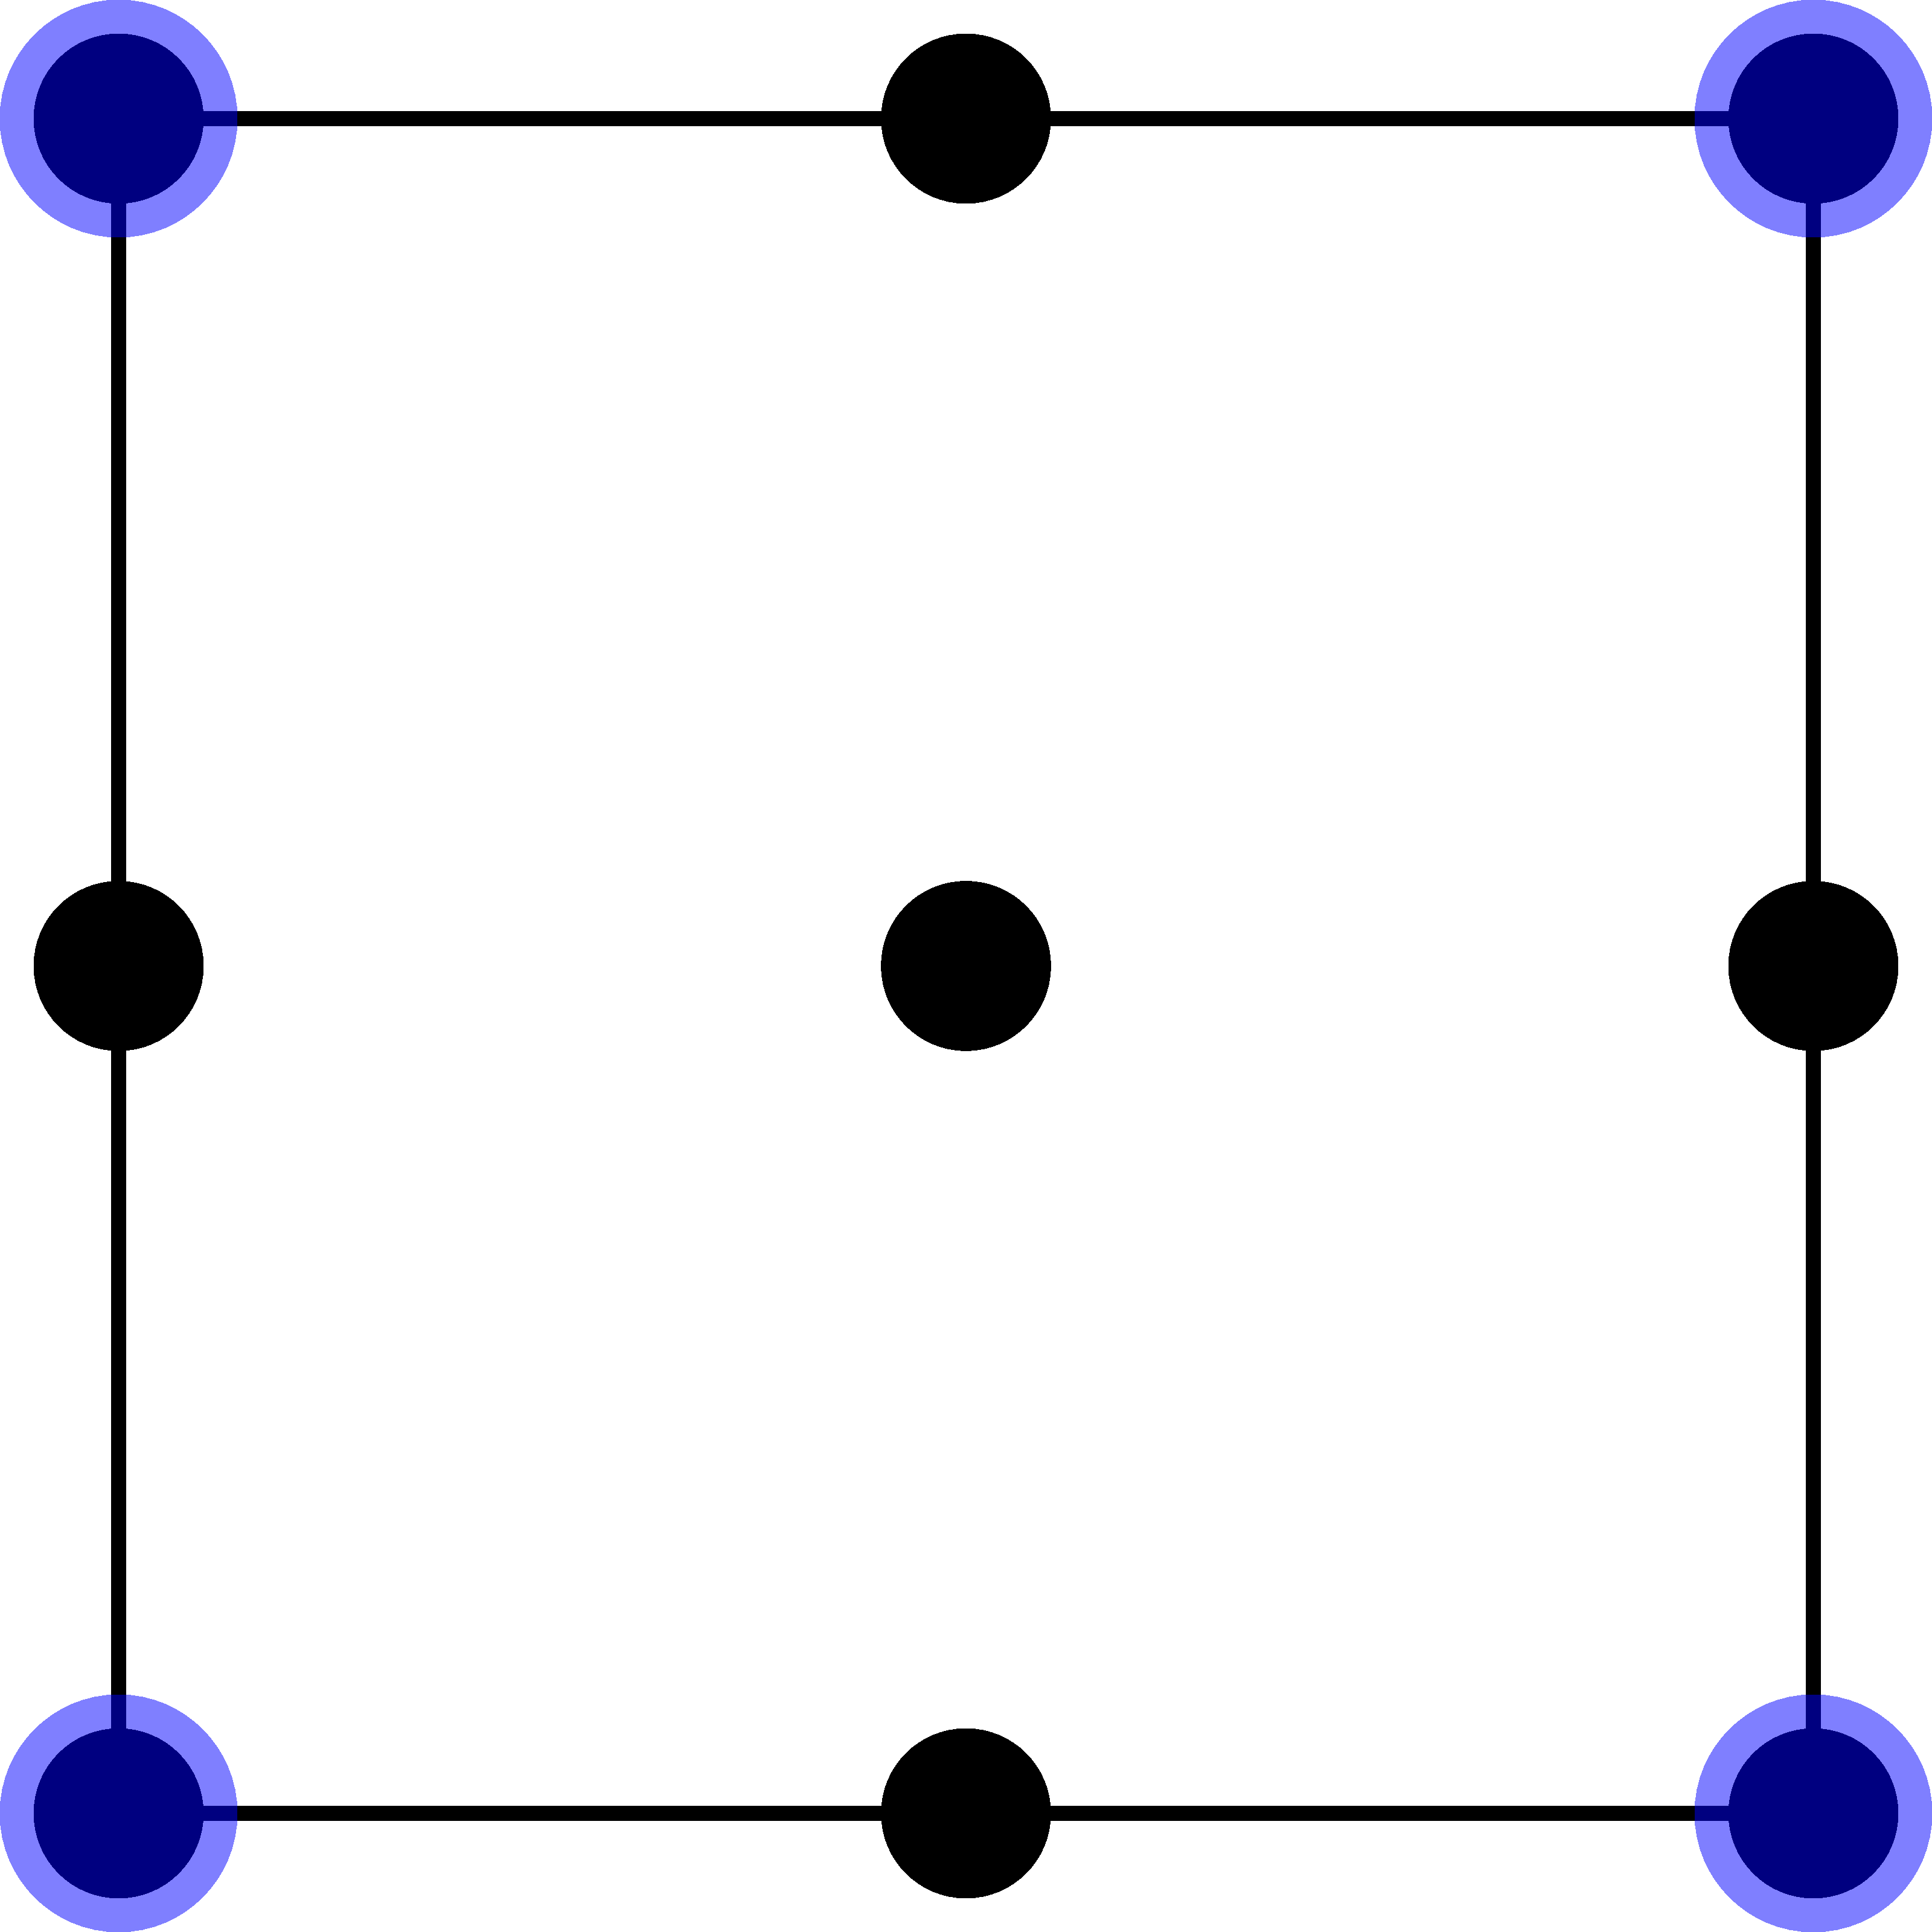
\includegraphics[width=0.1\textwidth]{png/TaylorHood.png}\\[-1.5ex]{\tiny Taylor--Hood($r=8$)}\\[1ex]}
% & \checkmark & \checkmark & \checkmark & \checkmark \\
% \parbox{0.2\textwidth}{\centering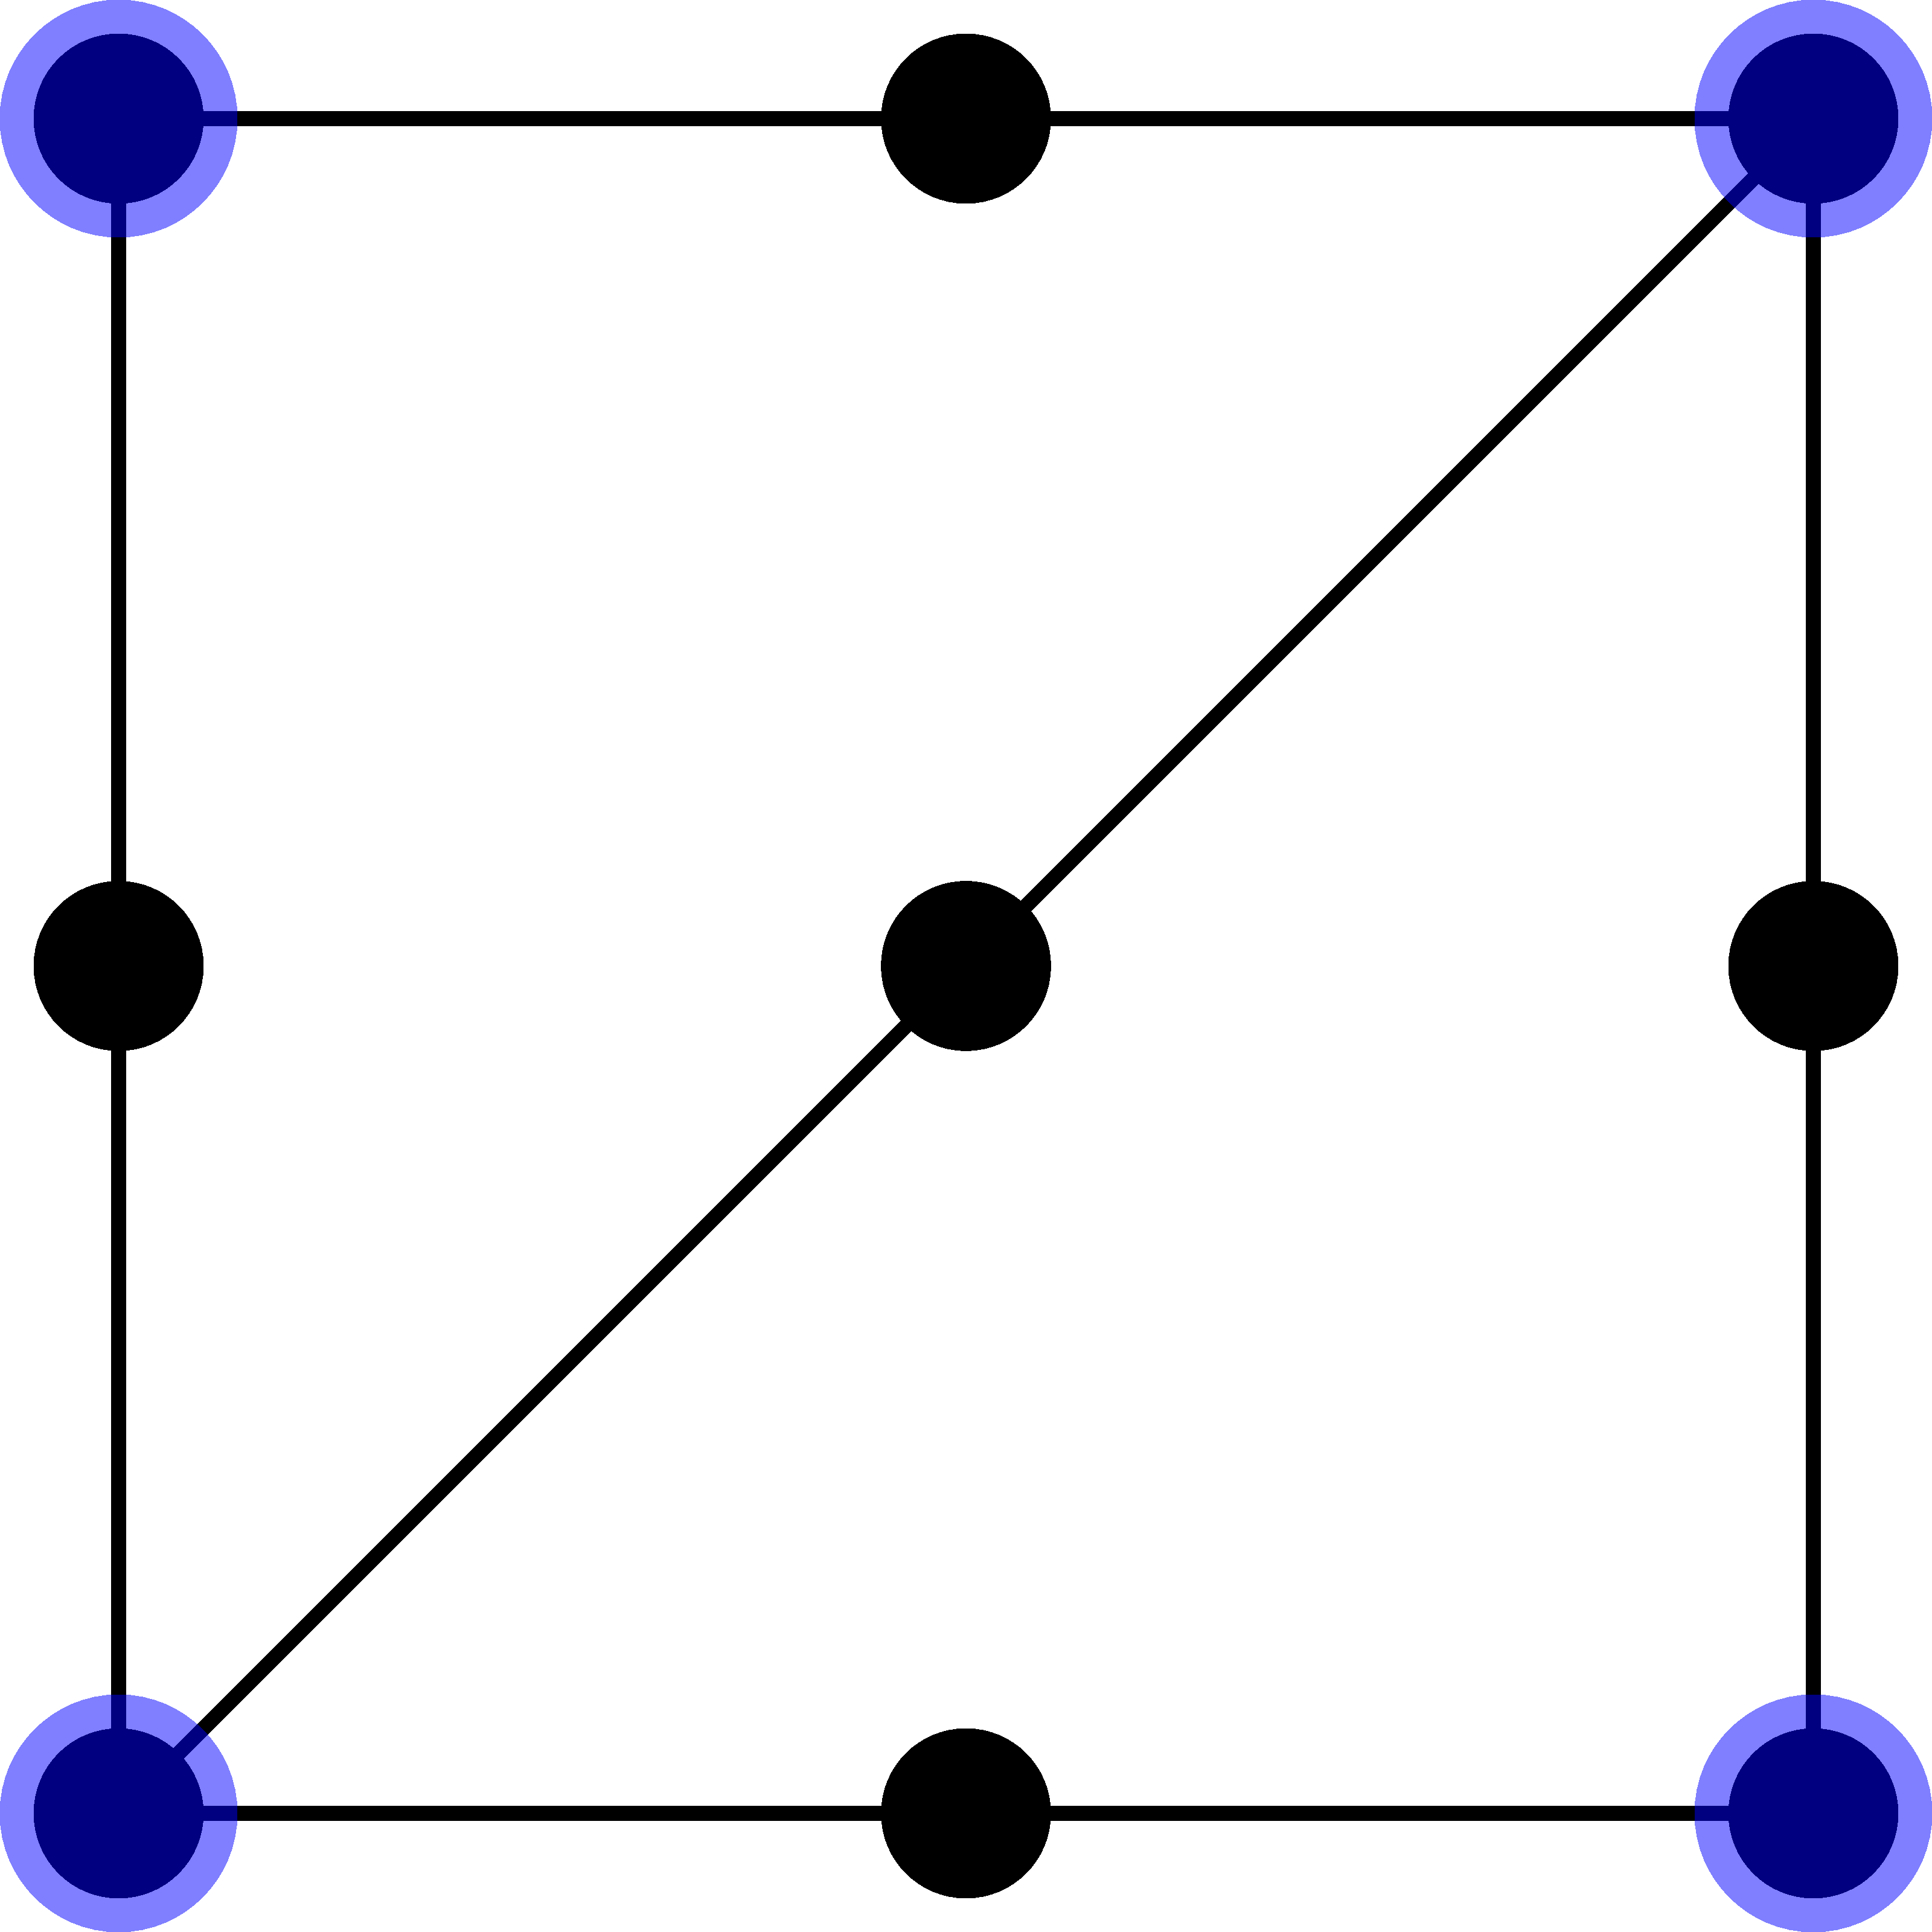
\includegraphics[width=0.1\textwidth]{png/mix_T6C3.png}\\[-1.5ex]{\tiny T6C3($r=\frac{8}{3}$)}\\[1ex]}
% & \checkmark & \checkmark &  & \checkmark \\
% \parbox{0.25\textwidth}{\centering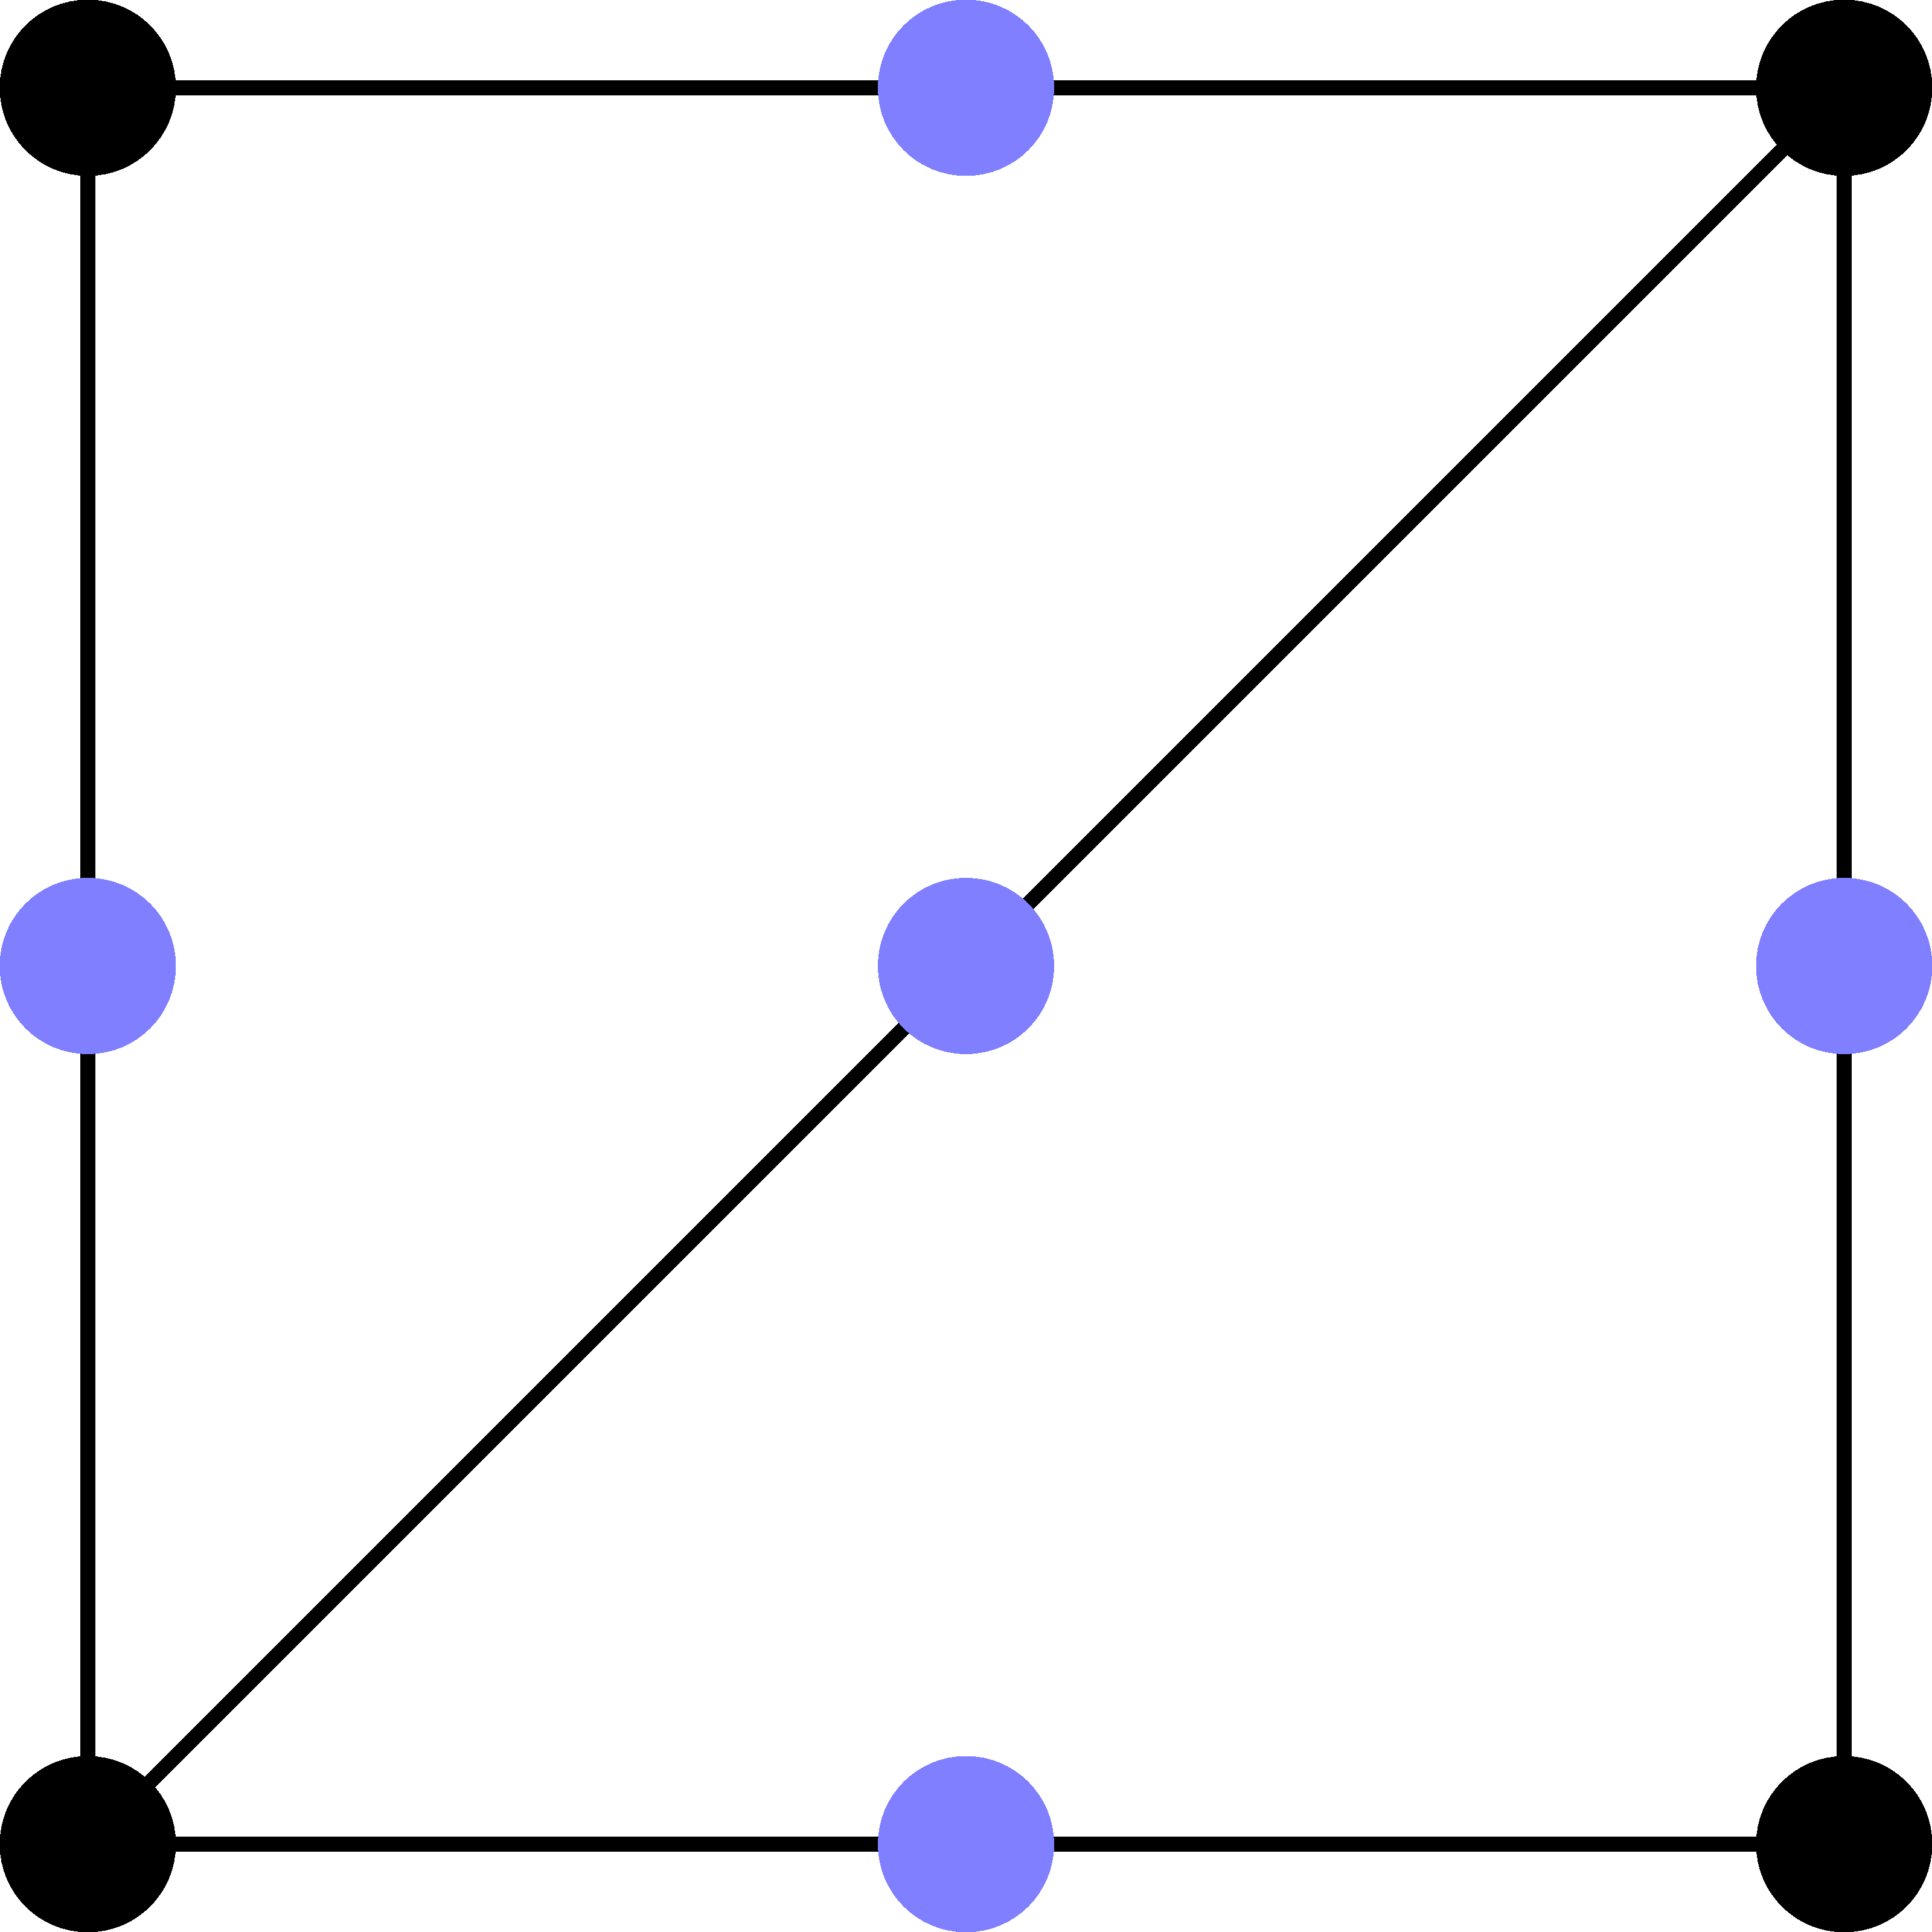
\includegraphics[width=0.1\textwidth]{png/CrouzeixRaviart.png}\\[-1.5ex]{\tiny Crouzeix--Raviart($r=4$)}\\[1ex]}
% & \checkmark & \checkmark &  & \checkmark \\
% \hline
% \multicolumn{5}{c}{
%     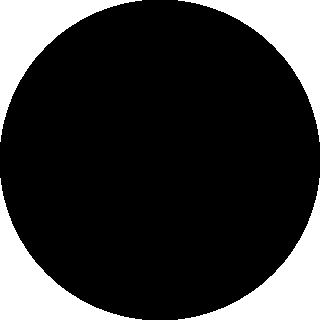
\includegraphics[width=5pt]{png/legend_u.png}
%     \scriptsize :Displacement node
%     \quad
%     
\includegraphics[width=5pt]{png/legend_p2.png}
%     \scriptsize :Discontinuous pressure node
%     \quad
%     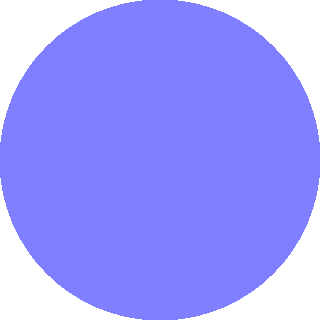
\includegraphics[width=5pt]{png/legend_p.png}
%     \scriptsize :Continuous pressure node
% }\\
% \hline
% \end{tabular}
% \end{table}

